% Tdyssey course paper: draft skeleton (due one week after the talk).
% Build: see README.md in this folder. Local: cd paper && latexmk -pdf main.tex
% Every number below comes from presentation/data/ (CSV and tables/*.tex) or docs/LEARNING_FINDINGS.md and
% docs/DECISIONS.md (D040-D056). The decision-log entry behind a number is given in a LaTeX comment next to it.
% Red [TODO: ...] markers show what is still missing; remove them all before submission.
\documentclass[10pt,twocolumn,letterpaper]{article}

\usepackage[T1]{fontenc}
\usepackage{lmodern}
\usepackage{microtype}
\usepackage[margin=0.75in,columnsep=0.25in]{geometry}
\usepackage{amsmath,amssymb}
\usepackage{graphicx}
\usepackage{booktabs}
\usepackage{adjustbox}
\usepackage{xcolor}
\usepackage{tikz}
\usetikzlibrary{arrows.meta,positioning}
\usepackage[numbers,sort&compress]{natbib}
\usepackage[colorlinks=true,linkcolor=blue!50!black,citecolor=blue!50!black,urlcolor=blue!50!black]{hyperref}

% Red TODO marker (robust, so it also works inside captions).
\DeclareRobustCommand{\todo}[1]{\textcolor{red}{[TODO: #1]}}

\title{Tdyssey: Adapting a T-Only Visuomotor Diffusion Policy to 26 Letter Shapes without New Human Demonstrations}
\author{\todo{three authors}}
\date{CS5478 course project \quad \todo{date}}

\begin{document}
\maketitle

% =====================================================================================================================
\begin{abstract}
The official camera-based Diffusion Policy for the PushT task was trained on 206 human demonstrations of a single
T-shaped block. Across 27 block shapes (the 26 capital letters and a narrower T) it succeeds in 3.7\% of fresh test
scenes. We adapt it to all 27 shapes without collecting any new human demonstrations. A planner that reads the
simulator state and plans inside a world model learned from non-expert machine rollouts acts as a teacher; the camera
policy is trained to copy the teacher's intended 16-step plans and is then refined in correction rounds, in which the
policy drives and the teacher relabels the states it visits. On 300 fresh scenes per shape, success over the 27
trained shapes rises from 3.7\% to 33.4\% with the original $96\times96$ camera and to 33.8\% with a $192\times192$
camera; on six shapes never used in training it rises from 1.2\% to 4.7--5.9\%. Before this recipe we tried
reinforcement-learning fine-tuning in the simulator, best-of-$N$ reranking with the true simulator, backpropagation
through the world model, and weight blending; we report these negative results and diagnose why the first one
failed. Most remaining failures end close to the goal but miss the 95\% coverage needed for success.
\todo{final pass on the abstract once results and page budget are fixed}
\end{abstract}

% =====================================================================================================================
\section{Introduction}
\label{sec:intro}

Visuomotor policies trained by behaviour cloning, such as Diffusion Policy~\citep{chi2023diffusion}, work well on the
task they were shown but carry little of that skill to a new object. The released PushT checkpoint is a clear case:
it solves the T in 42--46\% of fresh scenes and a slightly narrower T in 37--42\%, but on the other 25 capital letters it
succeeds in 0--9\% of scenes, 3.7\% on average over all 27 trained shapes (Table~\ref{tab:headline}). Collecting new
human demonstrations for every shape is the obvious fix and the one we rule out.

We ask whether one camera policy can be adapted to many new object shapes using only machine-generated interaction.
We set three rules: no new human demonstrations, teleoperation or success labels; the deployed policy sees only what
the original sees (two camera frames and the pusher position); and exact simulator state may be used only to create
training data, and is disclosed (Section~\ref{sec:limits}). The robot and the task stay the same; only the pushed
object changes (Fig.~\ref{fig:shapes}).

Our recipe has four parts (Fig.~\ref{fig:method}): a structured world model of pushing learned from noisy rollouts of
the original policy; a sampling planner that uses this model and the simulator state as a teacher; a camera student
trained with the official Diffusion Policy recipe to copy the teacher's \emph{intended} plans; and correction rounds
in the style of DAgger~\citep{ross2011dagger}. We grew the shape set in three stages (5, 10 and 27 shapes) and tested
each stage on fresh scenes chosen before the run.

Contributions: (i) a teacher--student recipe that raises success over 27 shapes from 3.7\% to 33.4\% (96~px camera)
without new human demonstrations; (ii) a fresh-scene test protocol with pre-registered candidates and paired
intervals; (iii) negative results for forward-process RL fine-tuning, simulator reranking, gradient-based planning
and weight blending, with a diagnosis of the RL training signal; (iv) an analysis of what limits success: final
alignment, plan commitment length and per-shape training budget.
\todo{tighten to one paragraph per point; decide whether to state the 34.8\% round-50 number in the intro}

\begin{figure*}[t]
  \centering
  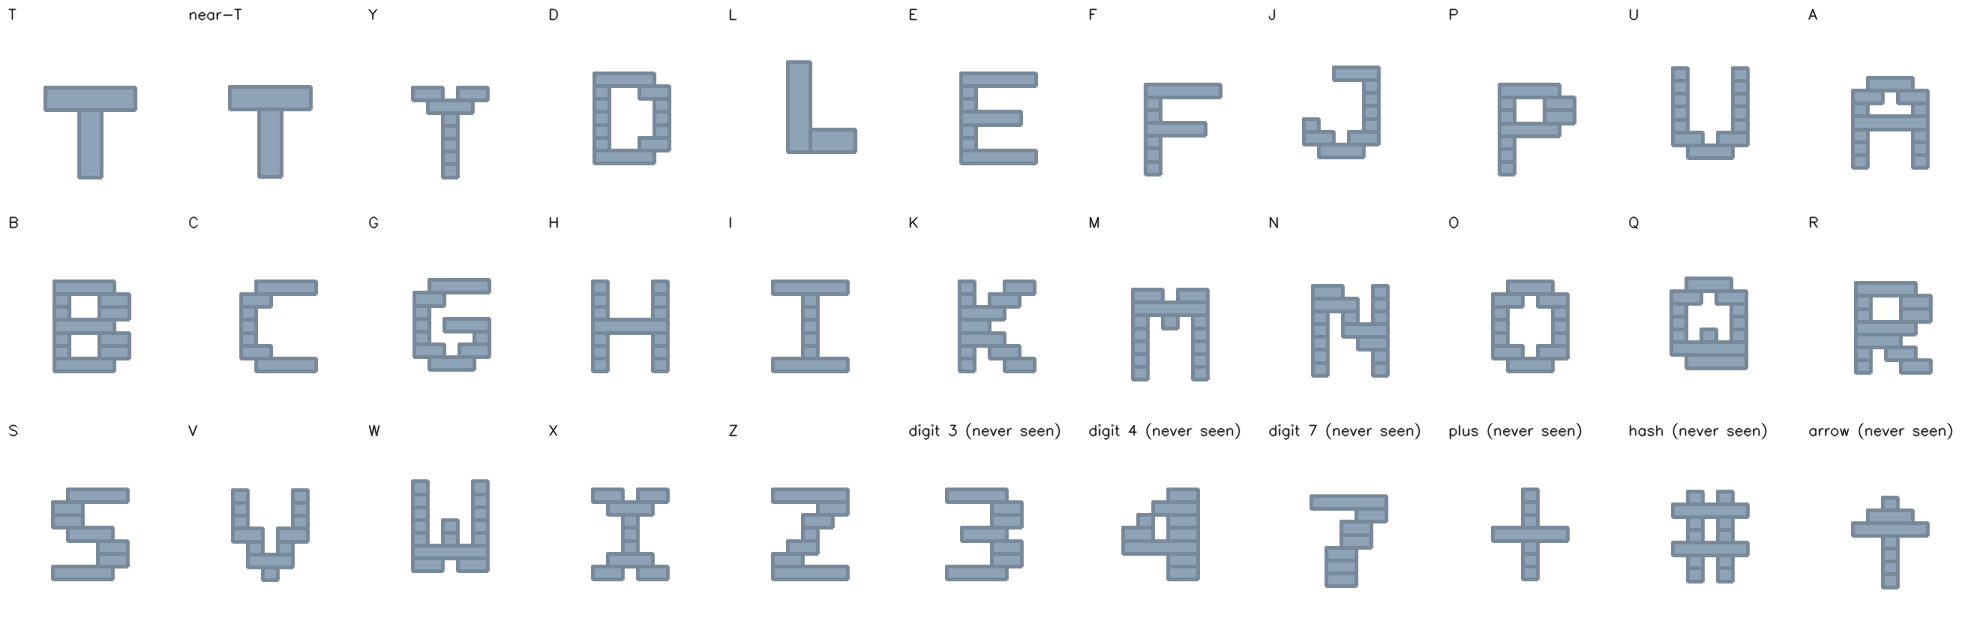
\includegraphics[width=\textwidth]{../images/shape_gallery_33_upright.png}
  \caption{The 33 shapes: the 26 capital letters and a narrower T (near-T) are trained; the six shapes in the last
  group (digits 3, 4, 7, plus, hash and arrow) are held out and used only in the final test.
  \todo{check the gallery's order and labels match this caption}}
  \label{fig:shapes}
\end{figure*}

% =====================================================================================================================
\section{Related work}
\label{sec:related}

\paragraph{Diffusion policies and imitation.}
Diffusion Policy~\citep{chi2023diffusion} predicts a short sequence of future actions by iterative denoising
(DDPM~\citep{ho2020ddpm}; DDIM~\citep{song2021ddim} for faster sampling) and reported strong results on PushT, a
task introduced with Implicit Behavioral Cloning~\citep{florence2021implicit}. Studies of offline imitation such as
robomimic~\citep{mandlekar2021robomimic} show how strongly results depend on data quality and evaluation. We keep the
released checkpoint, its observation interface and its training recipe unchanged and change only the data.
\todo{one sentence on action chunking and why 8 of 16 steps are executed}

\paragraph{RL fine-tuning of diffusion policies.}
DPPO~\citep{ren2025dppo} applies policy gradients to the denoising chain, DDPO~\citep{black2024ddpo} does the same for
image models, and DSRL~\citep{wagenmaker2025dsrl} instead runs RL over the policy's input noise and leaves its weights
fixed. Forward-process methods such as DiffusionNFT~\citep{zheng2026diffusionnft} and
AdvantageFlow~\citep{kveton2026advantageflow} weight the ordinary denoising loss by a reward or advantage signal and
need no likelihoods. Our attempt in this family failed because, with chunked actions and long episodes, the score of
one candidate plan was dominated by the randomness of the plans that followed it (Section~\ref{sec:negative}); we
expect the same problem for other methods that score one action chunk by the return that follows it. \todo{cite PPO~\citep{schulman2017ppo} only if the DPPO comparison needs it}

\paragraph{Privileged teachers and DAgger.}
Training a sensor-based student from a teacher with privileged state is well established: guided policy
search~\citep{levine2016end}, PLATO~\citep{kahn2017plato}, Learning by Cheating~\citep{chen2019lbc}, asymmetric
actor-critic~\citep{pinto2018asymmetric} and quadruped locomotion~\citep{lee2020quadruped}. DAgger~\citep{ross2011dagger}
reduces the mismatch between teacher and student states by letting the student drive and the teacher relabel. Our
setting differs in that the student is a pretrained diffusion policy with action chunks, which makes the choice of
label (intended plan versus executed actions) matter a great deal (Section~\ref{sec:ablations}).

\paragraph{World models for planning.}
Learned dynamics models are used for sampling-based planning (PETS~\citep{chua2018pets}, PlaNet~\citep{hafner2019planet},
TD-MPC2~\citep{hansen2024tdmpc2}; CEM~\citep{rubinstein1999cem,deboer2005tutorial} and MPPI~\citep{williams2017mppi}
as optimizers) and for policy learning in imagination~\citep{ha2018worldmodels,hafner2020dreamer,janner2019mbpo}.
GPC~\citep{qi2025gpc} ranks and refines a generative policy's proposals with a predictive world model at test time.
SuperMimic~\citep{liao2026supermimic} trains a policy by backpropagating through a learned differentiable world model;
\citet{suh2022differentiable} show that gradients through contact can be poorly behaved, which matches our
failure with this approach in planar pushing~\citep{mason1986mechanics}. We use the world model only inside a
privileged planner whose behaviour is distilled into the camera policy.

\paragraph{Generalist manipulation.}
Large multi-task policies (RT-1~\citep{brohan2023rt1}, Octo~\citep{octo2024}, OpenVLA~\citep{kim2024openvla},
$\pi_0$~\citep{black2025pi0}) gain breadth from large, diverse human datasets. We study the opposite end: how far one
narrow checkpoint can be extended with machine-generated data alone. \todo{one sentence on weight interpolation,
WiSE-FT~\citep{wortsman2022wiseft}, if Section~\ref{sec:negative} keeps the blending result}

% =====================================================================================================================
\section{Setup}
\label{sec:setup}

\paragraph{Task and simulator.}
We use the original planar PushT simulator released with Diffusion Policy~\citep{chi2023diffusion}, unchanged except
for the object. A disk-shaped pusher, moved by a PD controller towards commanded target positions, pushes a rigid
block in a $512\times512$ arena towards a fixed goal pose. With $B_t$ the block's footprint and $G$ the goal's, the
goal coverage at control $t$ is
\begin{equation}
  c_t = \frac{|B_t \cap G|}{|G|}, \qquad \text{success} \;\Leftrightarrow\; \max_{t \le 300} c_t > 0.95 .
  \label{eq:success}
\end{equation}
The episode ends at success or after 300 controls; we also report final coverage (at the end of the episode) and
peak coverage (its maximum). We keep the original success threshold.

\paragraph{Shapes.}
T and near-T keep the original mass, inertia and centre-of-mass convention; near-T shortens the T's top bar from 120
to 108 simulator pixels. The other capitals are built from a $5\times7$ block pattern (120~px tall, 100~px wide),
except L, which has its own definition (a 120~px stem and a 90~px foot, 30~px thick); each is one rigid body with
mass 1 and uniform-density inertia. Rendering, collision and reward all use the same rectangles, and overlap scoring handles the half-turn symmetry of H, I, O, S, X
and Z. The six held-out shapes (digits 3, 4 and 7, plus, hash, arrow) use the same block system, are one connected
piece each, and were fixed before the 27-shape run; they were never used for training, data collection, world-model
fitting or tuning. % D051
\todo{state that letter shapes change both appearance and dynamics, so results do not isolate visual recognition}

\paragraph{Policy.}
The baseline is the released RSS~2023 visual CNN Diffusion Policy checkpoint for PushT, trained on 206 human
demonstrations of the T only. It observes the two most recent $96\times96$ camera frames (cropped to $84\times84$)
and the pusher position, predicts 16 future pusher targets with 100 DDPM denoising steps, executes 8 of them, and
plans again. All our students keep this interface; the $192\times192$ students change only the camera resolution,
which is a sensor change and is reported separately (Fig.~\ref{fig:camera}).
\todo{one sentence on the architecture (ResNet-18 encoder~\citep{he2016resnet}, 1-D temporal
U-Net~\citep{ronneberger2015unet}); check parameter count against the 251M action network quoted in Table~\ref{tab:labels}}

\begin{figure}[t]
  \centering
  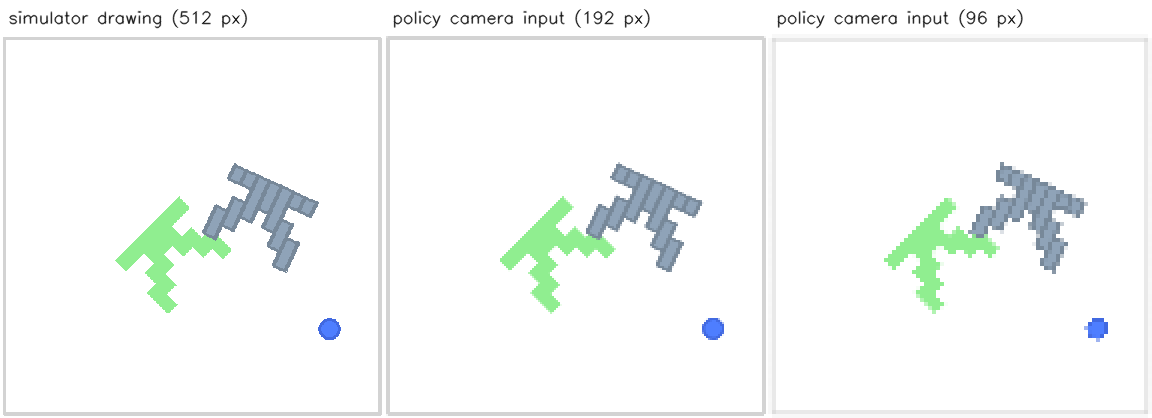
\includegraphics[width=\columnwidth]{../images/camera_views_512_192_96.png}
  \caption{What each policy sees: the simulator frame ($512\times512$), the $192\times192$ side-experiment camera and
  the original $96\times96$ camera. One 96~px camera pixel spans about 5 simulator pixels.}
  \label{fig:camera}
\end{figure}

\paragraph{Scene pools and test protocol.}
Every scene comes from a seed $\text{base} + 20i$, and the pools in Table~\ref{tab:pools} never overlap. Checkpoints
were picked on 50 fixed validation scenes per shape. Every final test used a pool never used before; the candidate,
the rule that picked it, the pool and the analysis were fixed before the test ran, and all policies ran on the same
scenes with the same policy-noise seed. Success rates carry 95\% Wilson intervals~\citep{wilson1927probable}; changes
between policies are paired by scene, with a 95\% normal-approximation interval on the per-scene differences.
\todo{mention the one data-hygiene incident: reserved final-test seeds were used by a collector for seven rounds and
quarantined before any training (LEARNING\_FINDINGS, open problems)}

\begin{table}[t]
  \centering\small
  \caption{Scene pools (seed $= \text{base} + 20i$). Training scenes use $i < 60{,}000$ of the 800,000 pool, so they
  stay below the first fresh pool. \todo{verify every row against docs/DECISIONS.md}}
  \label{tab:pools}
  \begin{adjustbox}{max width=\columnwidth}
  \begin{tabular}{lrrl}
    \toprule
    Use & Base seed & Scenes/shape & Shapes \\
    \midrule
    Validation (checkpoint picking) & 400{,}000 & 50 & trained \\
    World-model and dynamics data & 600{,}000 & -- & trained \\
    Teacher demos, correction rounds & 800{,}000 & varies & trained \\
    Test, 5 shapes, round 4 & 7{,}000{,}000 & 1000 & 5 \\        % D046
    Test, 5 shapes, round 7 & 8{,}000{,}000 & 1000 & 5 \\        % D047
    Test, 10 shapes & 9{,}000{,}000 & 1000 & 10 \\                % D049, D050
    Final test, 27 + 6 shapes & 10{,}000{,}000 & 300 & 33 \\      % D051
    Test, 17 untrained capitals & 11{,}000{,}000 & 200 & 17 + T \\ % D052
    Round 50, steps executed & 12{,}000{,}000 & 200 & 33 \\       % D054, D056
    Blend tests (Section~\ref{sec:negative}) & 0.9M; 2M; 3M; 4M & 1000; 2000 & 5 \\ % D040-D043
    \bottomrule
  \end{tabular}
  \end{adjustbox}
\end{table}

% =====================================================================================================================
\section{What did not work}
\label{sec:negative}

We report these attempts because they shaped the final recipe and because each one failed for a measurable reason.
\todo{decide how much of this section moves to the appendix if the page limit is tight}

\paragraph{Forward-process RL in the simulator.}
We fine-tuned the policy with forward-process objectives in the style of DiffusionNFT and AdvantageFlow on batched
simulator rollouts. Eight runs of about one million controls each with low-rank updates~\citep{hu2022lora} and a
learning rate of $10^{-5}$ left the policy essentially unchanged. With full-weight updates, a learning rate of $10^{-4}$ collapsed by
update 25, $3\times10^{-5}$ took T success from 0.55 to 0.05 by update 75, and every dense run at $10^{-5}$ or above
ended with T between 0.00 and 0.30 (Fig.~\ref{fig:rl}, left). To find out why, we re-scored candidate plans with
independent follow-up noise: only 16--36\% of a candidate's score variance came from the candidate itself, and
split-half reliability was 0.14--0.29 (Fig.~\ref{fig:rl}, right). The update was mostly fitting noise, and with no
anchor to the starting policy the drift accumulated. \todo{one sentence on the T-retention term being about $10^{-4}$
of the loss and on the privileged value function ($R^2 = 0.64$) not ranking candidates better}

\begin{figure*}[t]
  \centering
  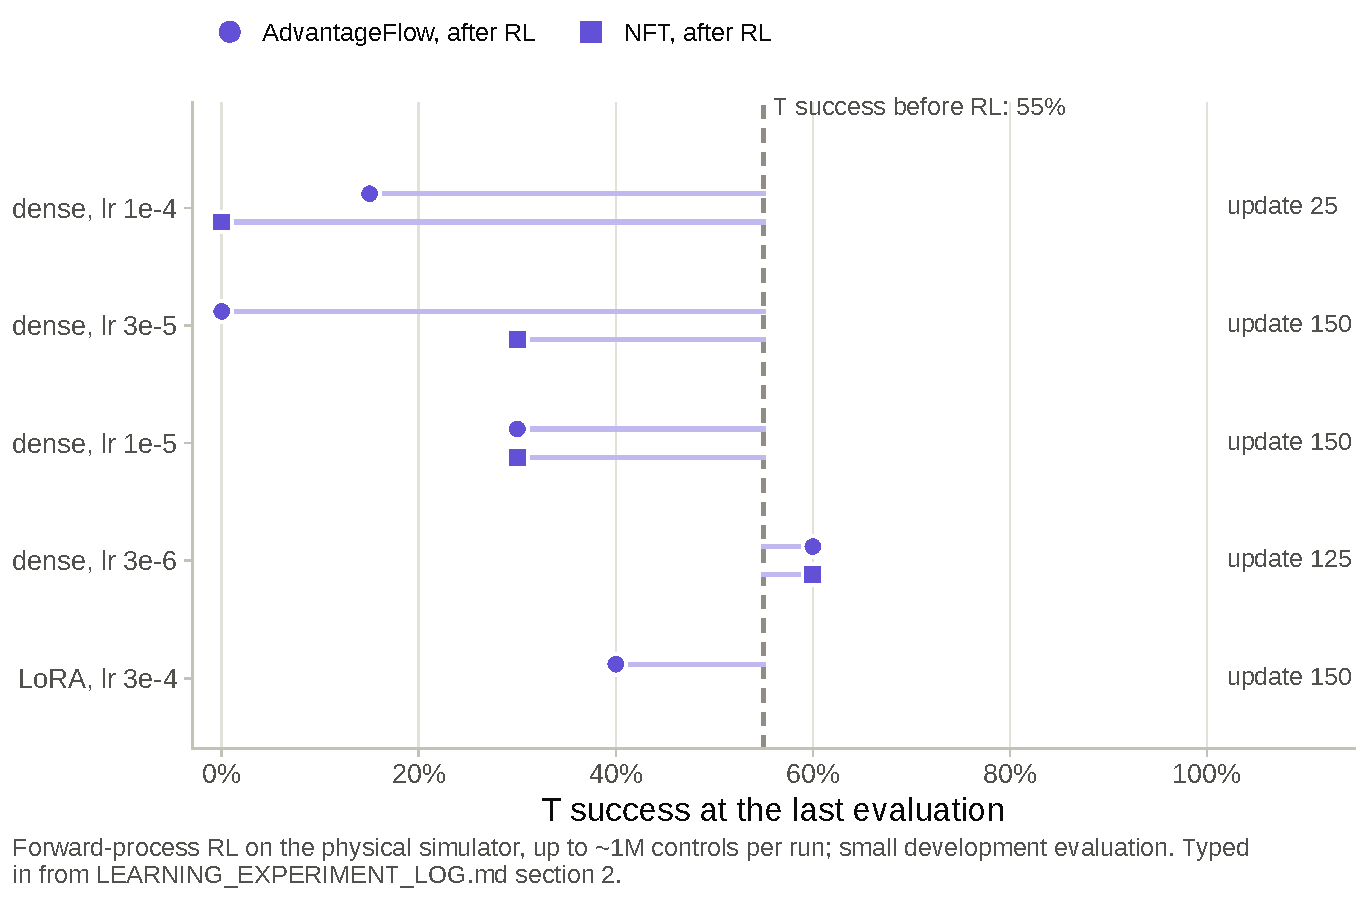
\includegraphics[width=0.49\textwidth]{../figures/rl_t_collapse.pdf}\hfill
  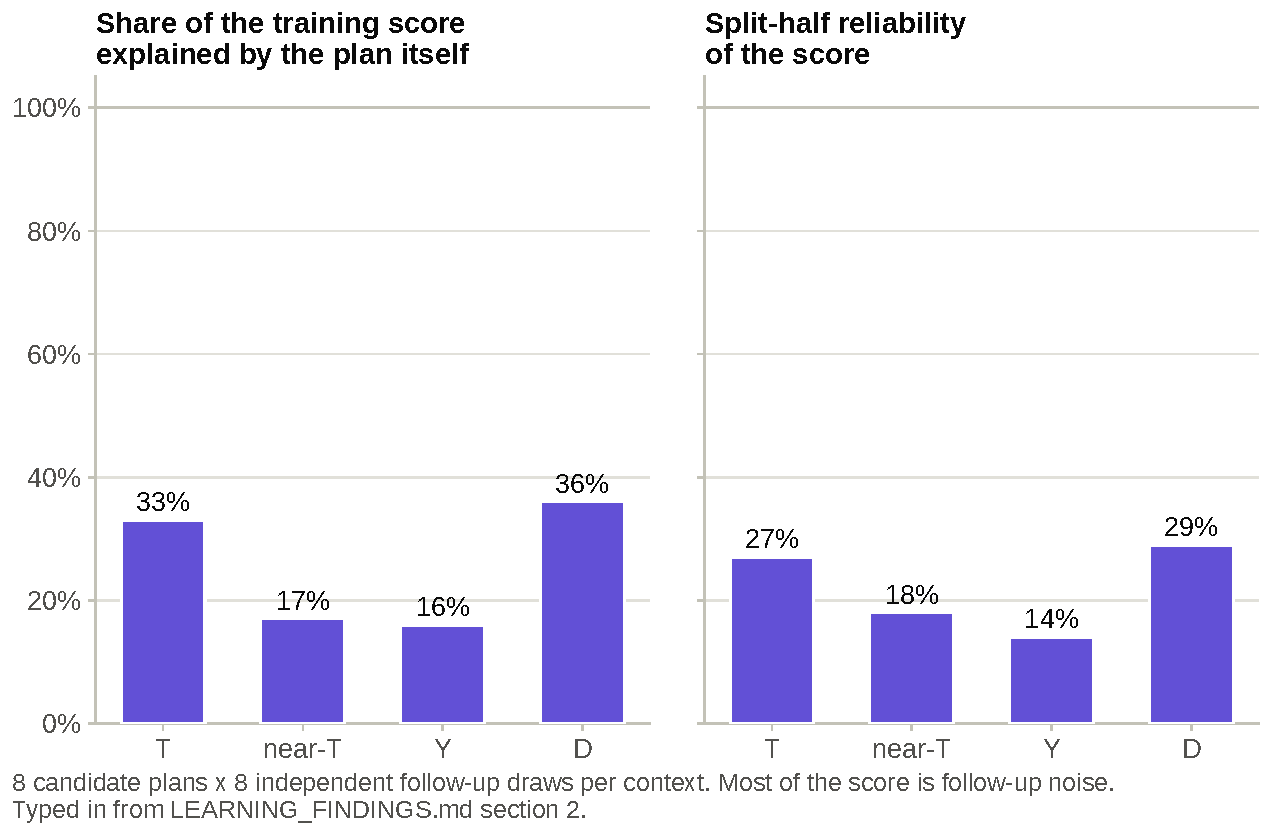
\includegraphics[width=0.49\textwidth]{../figures/rl_signal_variance.pdf}
  \caption{Forward-process RL. Left: T success before and after fine-tuning for each step size. Right: share of a
  candidate plan's score variance explained by the plan itself, and split-half reliability of the score; most of the
  training signal is noise from the plans that follow. Numbers typed in from the experiment log.}
  \label{fig:rl}
\end{figure*}

\paragraph{Best-of-$N$ with the true simulator.}
Sampling $N$ plans from the policy and committing to the one that does best in a replayed copy of the simulator is an
upper bound, not a policy, because it uses the true simulator at decision time. It helped a little (Y: 3 to 8
successes of 20 scenes), and imitating its choices stayed within test noise: the policy's own samples were too similar
to each other (spread about 0.02 in normalized action units) to contain new behaviour.
\todo{one sentence: world-model best-of-32 among policy samples gave a similar Y gain but still needs the true state}

\paragraph{Gradients through the world model.}
Training a deterministic state-based policy from scratch by backpropagating through 32 imagined steps of our world
model, in the style of SuperMimic~\citep{liao2026supermimic}, taught it to approach the block (gap 21 to 3.7~px) but
real-simulator coverage stayed at 0.04--0.12 after more than 500 iterations for every reward we tried. Gradients through contact appear to trap
it in local optima, as \citet{suh2022differentiable} report for planar pushing.

\paragraph{Distillation with an anchor, and weight blending.}
Distilling the planner into the policy with an anchor to the original weights first made every shape worse; training
the image encoder, longer training and student-driven data gave the first real D and L successes but cost 10--15 T
points. Blending student and original weights, $\theta_s = (1-s)\,\theta_{\text{orig}} + s\,\theta_{\text{student}}$
(as in WiSE-FT~\citep{wortsman2022wiseft}), recovered T. The best blend kept the original action network and half of
the student's image encoder; on 2000 fresh scenes per letter it raised Y from 8.6\% to 14.8\% and D from 0.3\% to
1.1\% with no significant T change, and it replicated on a third pool. % D042, D043
Because it keeps the original action network, it cannot carry most of the teacher's skill, so we moved to training a
full new policy. % D044
\todo{optional: Fig. final\_blends\_5shapes in the appendix (Fig.~\ref{fig:app-blends})}

% =====================================================================================================================
\section{Method}
\label{sec:method}

\begin{figure*}[t]
  \centering
  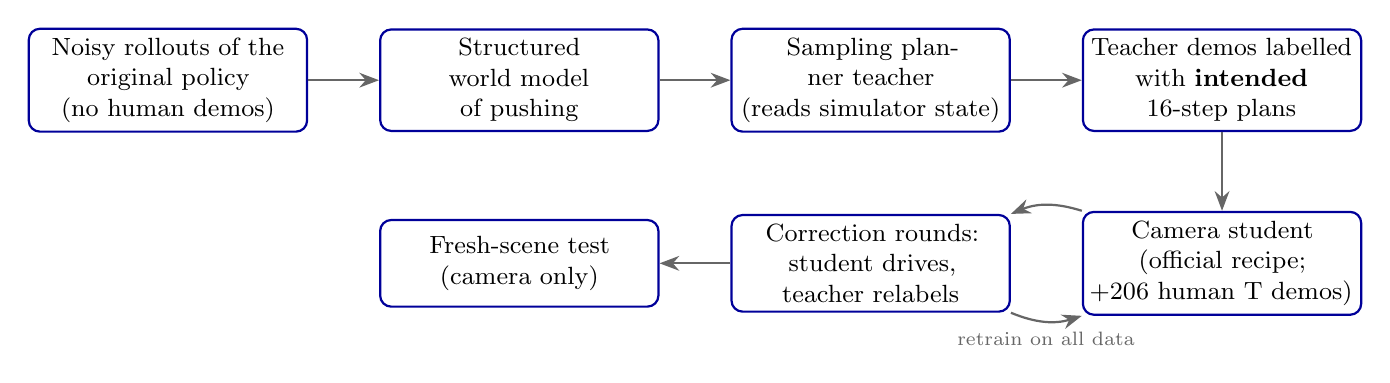
\begin{tikzpicture}[node distance=6mm and 9mm,
      box/.style={draw=blue!60!black, rounded corners, thick, align=center, minimum height=11mm, text width=33mm,
        font=\small},
      arr/.style={-{Stealth[length=2.5mm]}, thick, black!60}]
    \node[box] (data) {Noisy rollouts of the\\original policy\\(no human demos)};
    \node[box, right=of data] (wm) {Structured world model\\of pushing};
    \node[box, right=of wm] (teacher) {Sampling planner teacher\\(reads simulator state)};
    \node[box, right=of teacher] (demos) {Teacher demos labelled\\with \textbf{intended}\\16-step plans};
    \node[box, below=10mm of demos] (student) {Camera student\\(official recipe;\\+206 human T demos)};
    \node[box, left=of student] (rounds) {Correction rounds:\\student drives,\\teacher relabels};
    \node[box, left=of rounds] (test) {Fresh-scene test\\(camera only)};
    \draw[arr] (data) -- (wm);
    \draw[arr] (wm) -- (teacher);
    \draw[arr] (teacher) -- (demos);
    \draw[arr] (demos) -- (student);
    \draw[arr] (student.north west) to[bend right=20] (rounds.north east);
    \draw[arr] (rounds.south east) to[bend right=20] node[below, font=\scriptsize] {retrain on all data} (student.south west);
    \draw[arr] (rounds) -- (test);
  \end{tikzpicture}
  \caption{Overview. Exact simulator state is used only by the teacher to create training data; the tested policy sees
  two camera frames and the pusher position, exactly like the original. \todo{check the diagram renders; align
  with the slide version}}
  \label{fig:method}
\end{figure*}

\paragraph{Structured world model.}
The model predicts the block's motion from the current state and the commanded pusher targets. Only the block's motion
in contact is learned (an MLP in the block's frame); the pusher's PD dynamics are computed exactly (matching the
simulator to $10^{-4}$~px), the pusher-to-block distance comes from the letter's rectangles, and a contact gate sets the
block's motion to zero without contact. It is trained only on rollouts of the frozen original policy with Gaussian
action noise of 0, 10 and 25~px (1500 episodes and 431k controls for the first five shapes), with later versions
covering 10 and 27 shapes. Over 8 controls its median held-out contact error is 0.22--0.32~px on the first five shapes
(Fig.~\ref{fig:wm}). \todo{data sizes for world-model versions 2 and 3; mention the rare large errors near the arena
wall (1 in 20 windows off by 14~px or more)}

\begin{figure}[t]
  \centering
  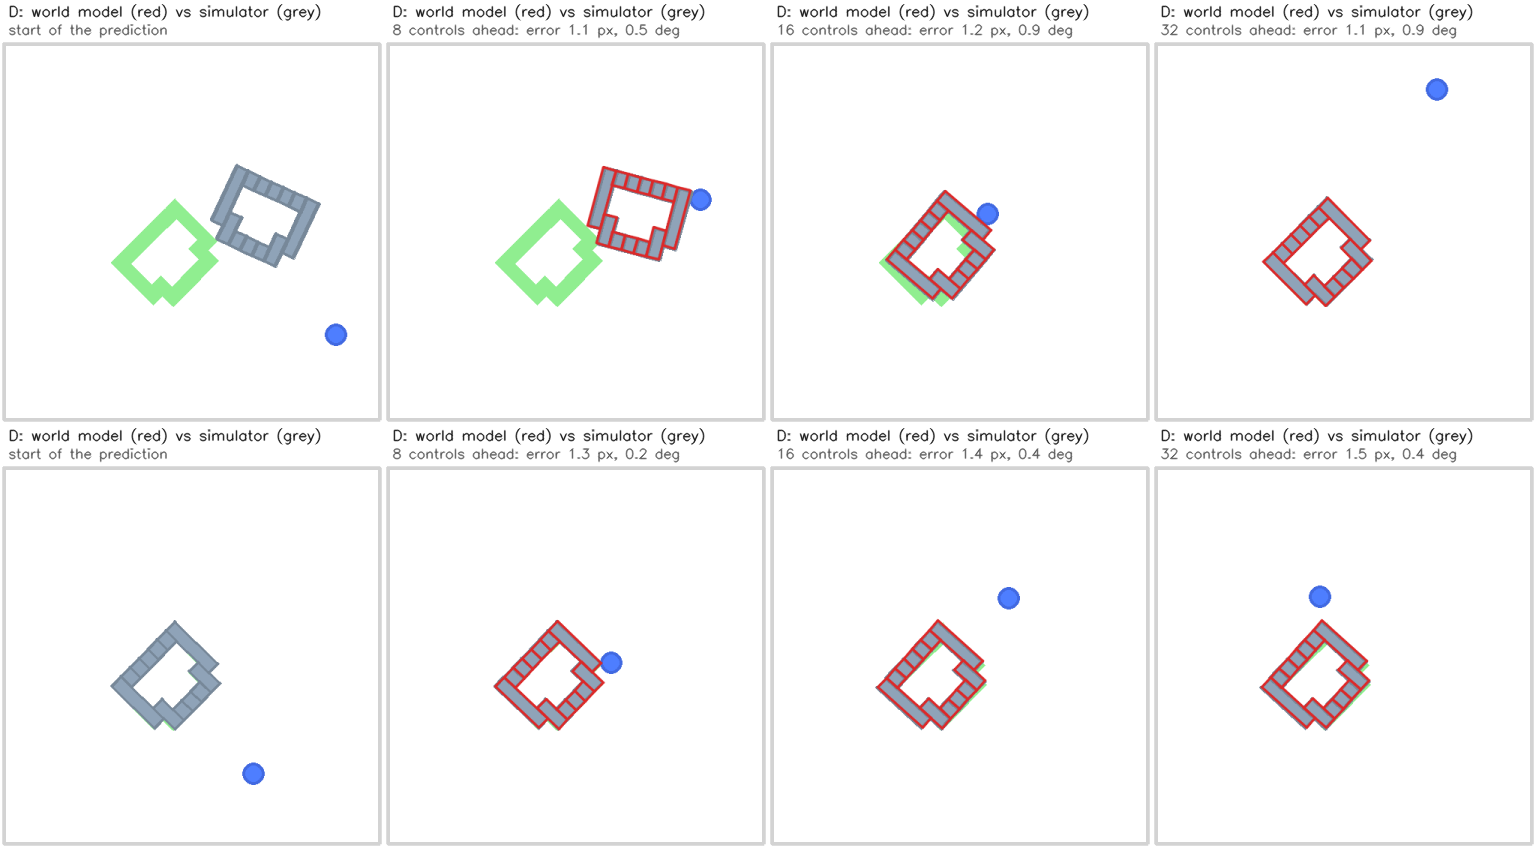
\includegraphics[width=\columnwidth]{../images/world_model/imagined_vs_real_D.png}
  \caption{World model (red) against the simulator (grey) for the same pusher targets, 8, 16 and 32 controls ahead (D).
  \todo{pick one of D, E, R, T; state the errors in the caption}}
  \label{fig:wm}
\end{figure}

\paragraph{Sampling planner teacher.}
At every control the teacher reads the block and pusher state, plans pusher targets inside the world model, and
executes the first target of the best plan. It combines the cross-entropy method~\citep{rubinstein1999cem} over smooth
random target paths with structured push candidates (move out to a safe circle, travel around the letter, push one
boundary point), keeps the single best sample rather than the elite mean, and scores plans by the pose error over
points spread across the letter's area with a sharp term for the last 1--2~px. Each of these choices removed one
measured cause of the planner stalling short of the goal. Reading the state with 1~px / 1$^\circ$ Gaussian noise made
it a better teacher (T 5 to 34 and L 11 to 39 successes of 50), probably because the noise breaks repeated near-miss
pushes. The teacher solves 390 of 500 validation scenes on ten shapes and 36--49 of 50 on each of the 17 later
letters (Fig.~\ref{fig:teacher}). \todo{planner settings: 256 samples, 4 CEM iterations, 24 elites, horizon 48 controls,
128 push candidates (mpc\_teacher.py); reconcile with the slide's ``about 1,150 candidate pushes per step''}

\begin{figure}[t]
  \centering
  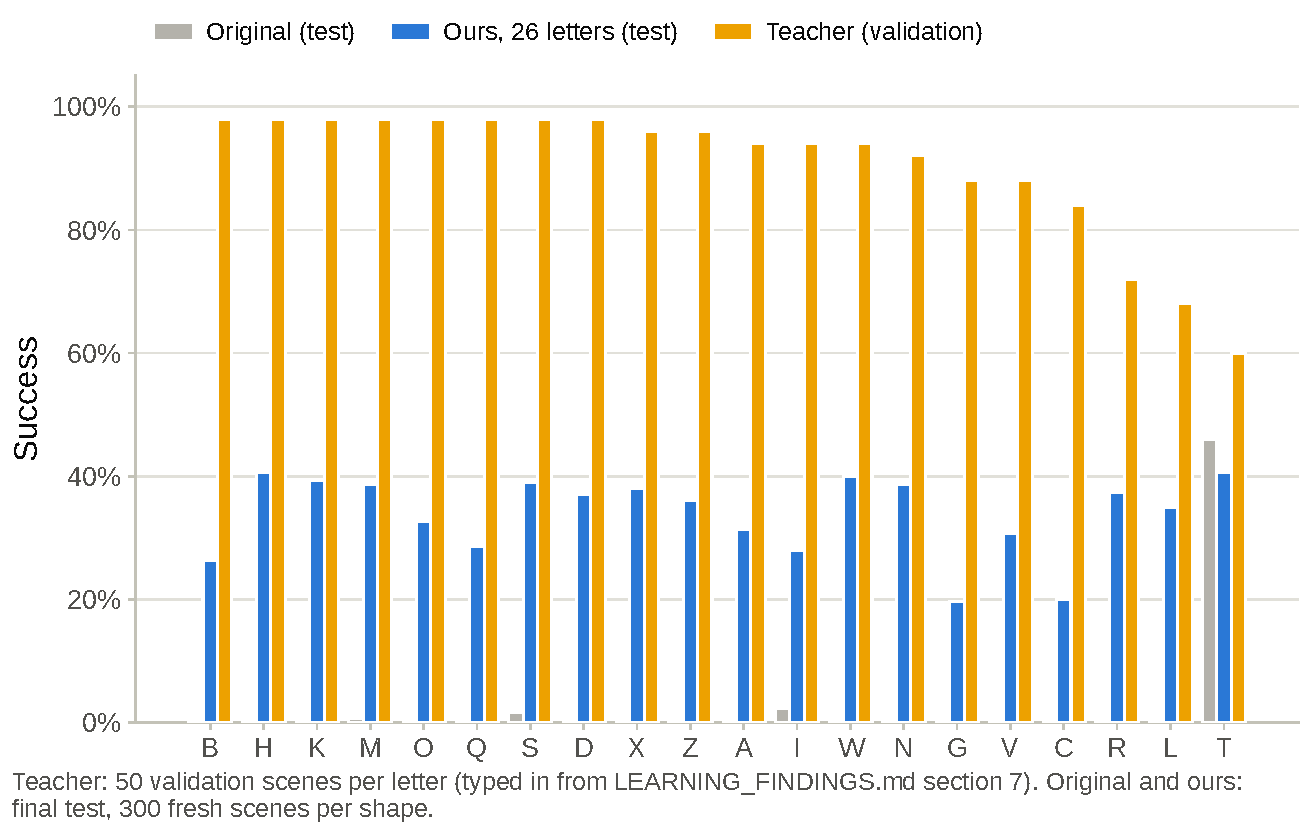
\includegraphics[width=\columnwidth]{../figures/method_teacher_success_26letters.pdf}
  \caption{Teacher (reads simulator state; validation scenes) against the original policy and our 27-shape camera
  student (final test) per letter. Teacher numbers typed in from the findings.}
  \label{fig:teacher}
\end{figure}

\paragraph{Intended-plan labels.}
The student predicts 16 targets and executes 8 open-loop, while the teacher replans every control. Labelling a state
with the 16 targets the teacher actually executed stitches together pieces of different plans; in the examples of
Fig.~\ref{fig:labels} the largest step between consecutive executed targets is 59--153~px, against 20--47~px within an
intended plan. We instead label each state with the teacher's intended plan: the first 16 targets of the best plan it
found at that state. In a matched test this raised validation successes from
77 to 129 of 1000, the largest single gain we measured (Table~\ref{tab:labels}).

\begin{figure}[t]
  \centering
  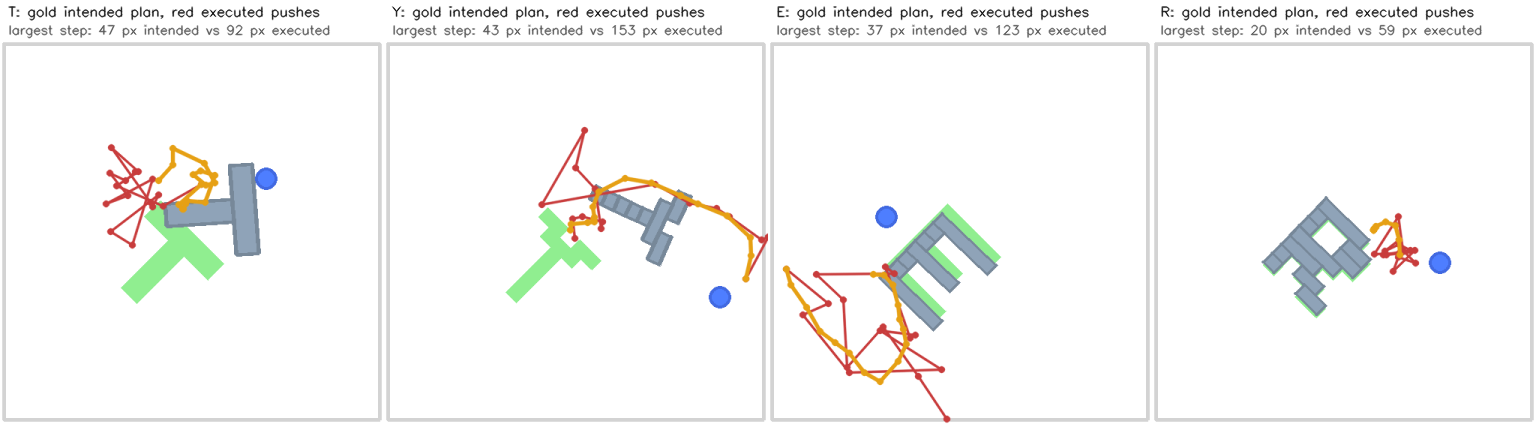
\includegraphics[width=\columnwidth]{../images/training_data/labels_intended_vs_executed.png}
  \caption{Label choice. Gold: the teacher's intended 16-step plan at one state. Red: the 16 pushes it actually
  executed while replanning every control. \todo{keep two of the four panels if space is short}}
  \label{fig:labels}
\end{figure}

\paragraph{Student and correction rounds.}
The student starts from the released checkpoint and is trained with the official Diffusion Policy recipe (denoising
loss~\citep{ho2020ddpm,chi2023diffusion}, image encoder and action network both trained, random-crop augmentation,
EMA weights, cosine learning rate) on every step of the teacher demonstrations, the original 206 human T
demonstrations and all correction data so far, with shapes balanced in every batch. In each correction round the
student chooses the next 8 controls with probability 0.7 (the teacher otherwise) on new training scenes; the teacher
labels every visited state with its intended plan, and the student is retrained on all data. \todo{learning rate
($10^{-4}$), batch size (256 implied by D053), demo counts per stage}

\paragraph{Stages and per-shape budget.}
We trained on 5 shapes (T, near-T, Y, D, L), then 10 (adding E, F, J, P, U), then 27 (adding the 17 other capitals),
each stage starting from the previous stage's student. With the ten-shape budget of 20k training steps per round,
27 shapes get 2.7 times less training each (190k instead of 512k samples per shape per round) and the 17 new letters
had 5--8 times fewer corrections; validation levelled off near 24\%. From round 14 we trained 54k steps per round and
collected 60 practice scenes per new letter (30 for the earlier ten), and validation rose to about 35\% by round 44
(Fig.~\ref{fig:budget}). % D053
\todo{rounds per stage and the selection rule for each candidate (D046-D051, D054)}

% =====================================================================================================================
\section{Results}
\label{sec:results}

\begin{figure*}[t]
  \centering
  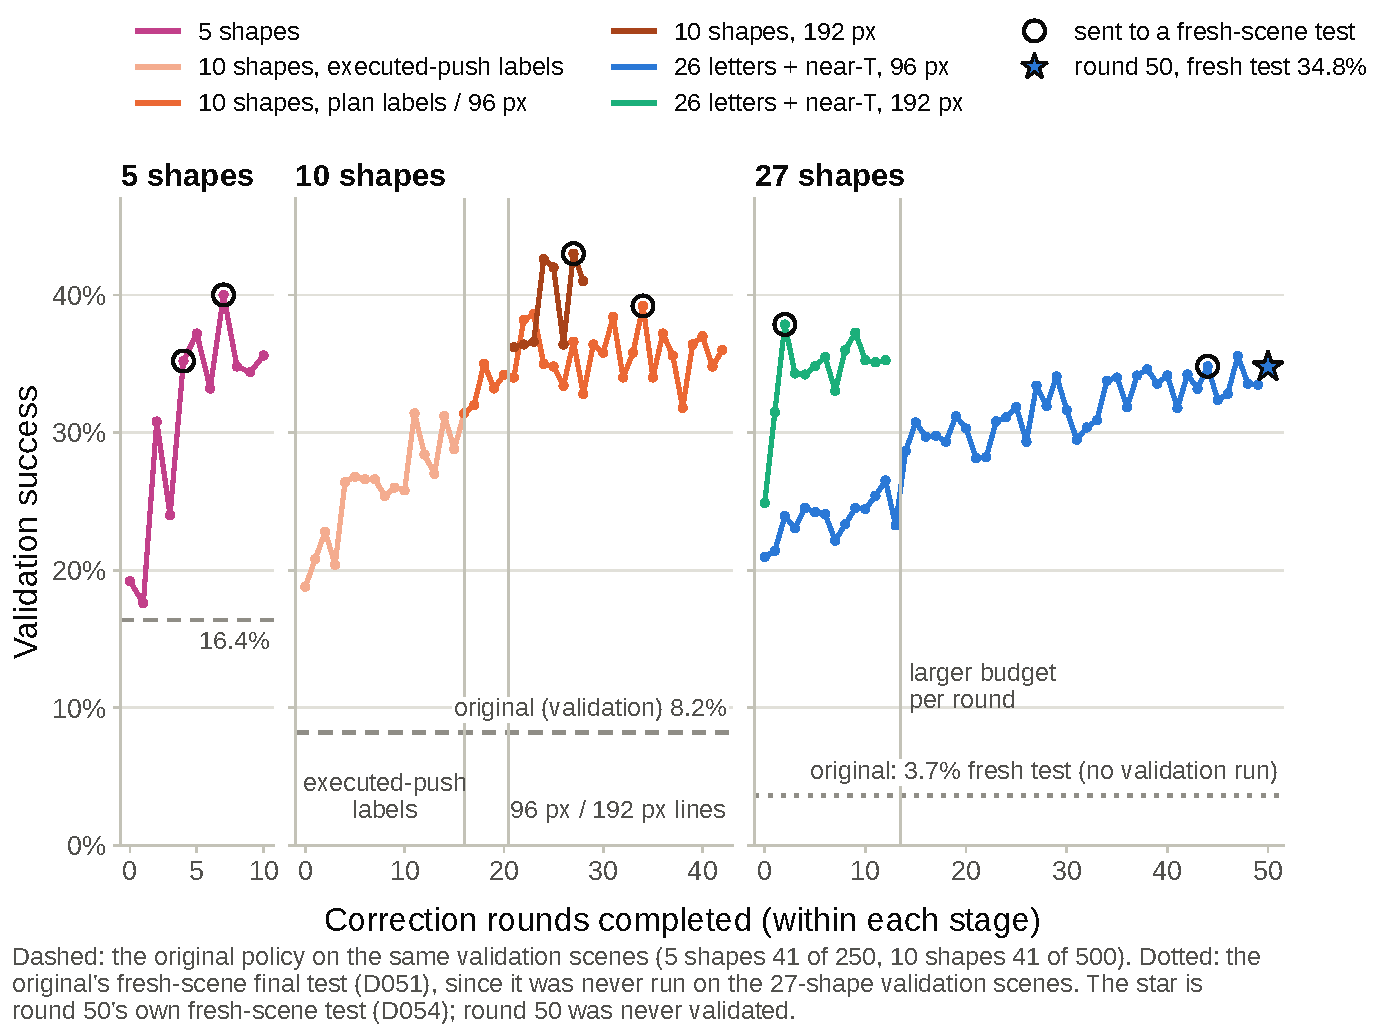
\includegraphics[width=0.85\textwidth]{../figures/curves_all_stages_panels.pdf}
  \caption{Validation success per correction round for the three stages (5, 10 and 27 shapes; 50 scenes per shape).
  Picked rounds are circled; the dashed line is the original policy. Validation numbers were used for picking
  checkpoints and are biased upward; all claims use the fresh-scene tests.}
  \label{fig:curves}
\end{figure*}

\paragraph{Training.}
Figure~\ref{fig:curves} shows validation success through the project. Each stage rises quickly in the first few
correction rounds and then flattens; in the ten-shape stage, 21 later validation tests averaged 179 of 500 with a
spread of 9.6, about what chance alone gives (10.7), and the same student tested twice on the same scenes flipped 211
of 500 outcomes. Extra rounds therefore change the true success rate slowly, and the fresh-scene tests below are the
only numbers we use for claims. \todo{one sentence on the 192~px line (best validation 511 of 1350 at round 2)}

\begin{figure}[t]
  \centering
  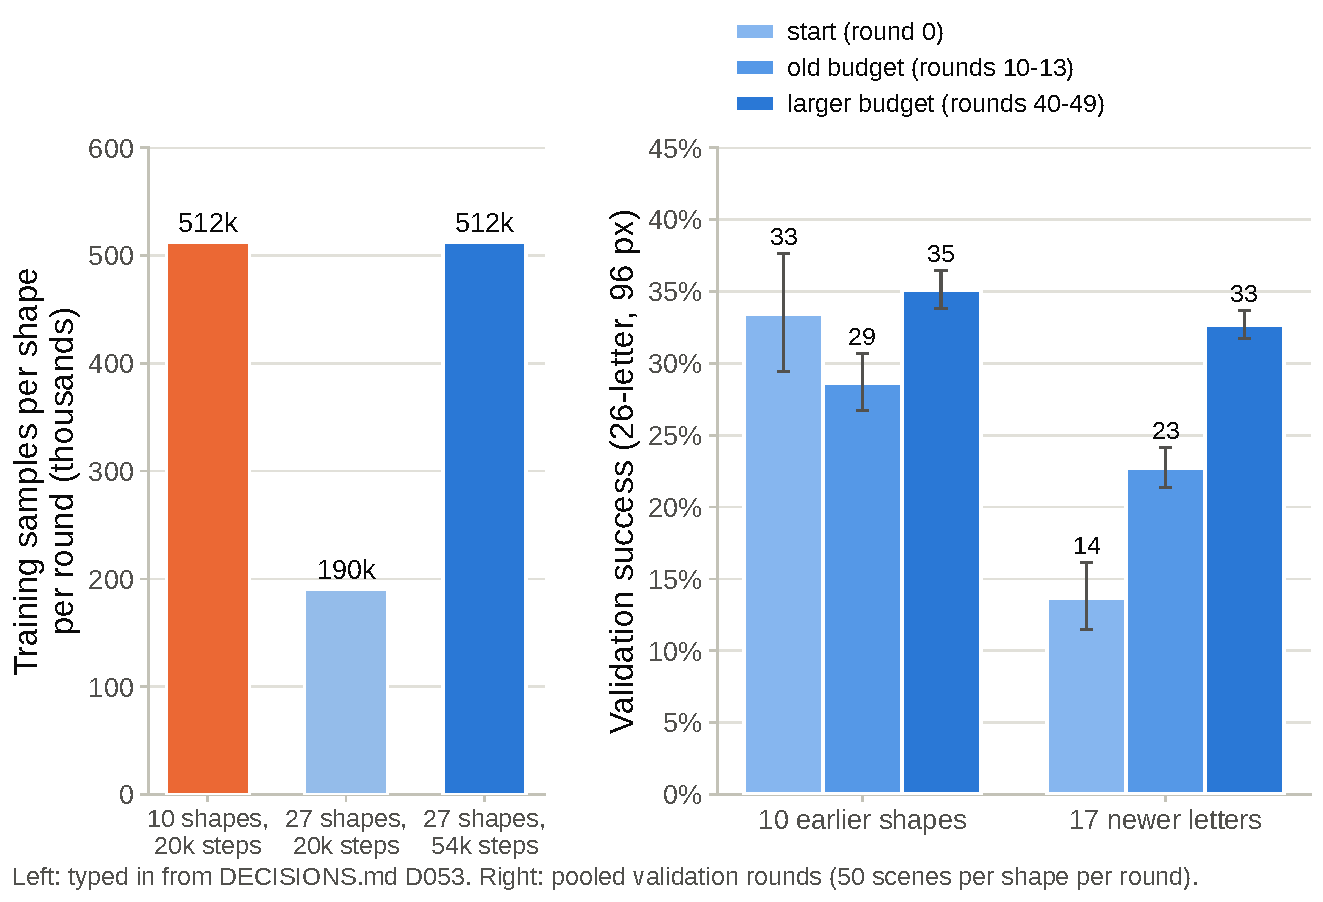
\includegraphics[width=\columnwidth]{../figures/analysis_budget.pdf}
  \caption{27-shape budget diagnosis: training samples per shape per round, and validation before and after the
  larger budget.}
  \label{fig:budget}
\end{figure}

\paragraph{Final test, 27 shapes.}
On 300 fresh scenes per shape (Table~\ref{tab:headline}), success over the 27 trained shapes rises from 3.7\% to
33.4\% (96~px; $+29.8$ points, 95\% interval $[+28.7, +30.9]$) and 33.8\% (192~px; $+30.1$ $[+29.0, +31.2]$). The ten
earlier shapes are unchanged by adding 17 letters (33.0\% with the ten-shape student, 33.7\% with the 27-shape one),
and the 17 new letters rise from 0.4\% to 33.2\%. Every trained shape improves except T and near-T
(Fig.~\ref{fig:dumbbell}); mean final coverage rises from 0.35 to 0.82. Six more correction rounds (round 50 against
the pre-registered round 44) added $+1.9$ points $[+0.1, +3.6]$ on a separate fresh pool, reaching 34.8\%
(Table~\ref{tab:r50}). % D051, D054
\todo{state explicitly that D051 (round 44) stays the pre-registered headline}

\begin{table*}[t]
  \centering
  \caption{Final test (pre-registered): success (\%) on 300 fresh scenes per shape, paired by scene; changes in
  points with 95\% intervals. ``10 shapes'' is the ten-shape student, which never trained on the 17 newer letters.}
  \label{tab:headline}
  \begin{adjustbox}{max width=\textwidth}
  % Generated by presentation/scripts/make_figures.py from presentation/data/*.csv. Needs \usepackage{booktabs}.

\begin{tabular}{lrrrr}
\toprule
Shapes & Original & Ours, 10 shapes & Ours, 26 letters & Ours, 26 letters (192 px) \\
\midrule
10 earlier shapes & 9.3 & 33.0 & 33.7 & 34.2 \\
17 newer letters & 0.4 & 6.4 & 33.2 & 33.5 \\
All 27 trained shapes & 3.7 & 16.3 & \textbf{33.4} & \textbf{33.8} \\
6 never-seen shapes & 1.2 & 2.8 & 4.7 & 5.9 \\
\midrule
Change vs.\ original, all 27 trained shapes & -- & +12.6 [+11.8, +13.5] & +29.8 [+28.7, +30.9] & +30.1 [+29.0, +31.2] \\
Change vs.\ original, 6 never-seen shapes & -- & +1.6 [+0.7, +2.4] & +3.5 [+2.4, +4.6] & +4.7 [+3.5, +5.9] \\
Final coverage, 27 trained shapes & 0.35 & 0.63 & 0.82 & 0.81 \\
\bottomrule
\end{tabular}
% Success %; final test, 300 fresh scenes per shape, paired by scene; differences in points with 95% intervals.

  \end{adjustbox}
\end{table*}

\begin{figure}[t]
  \centering
  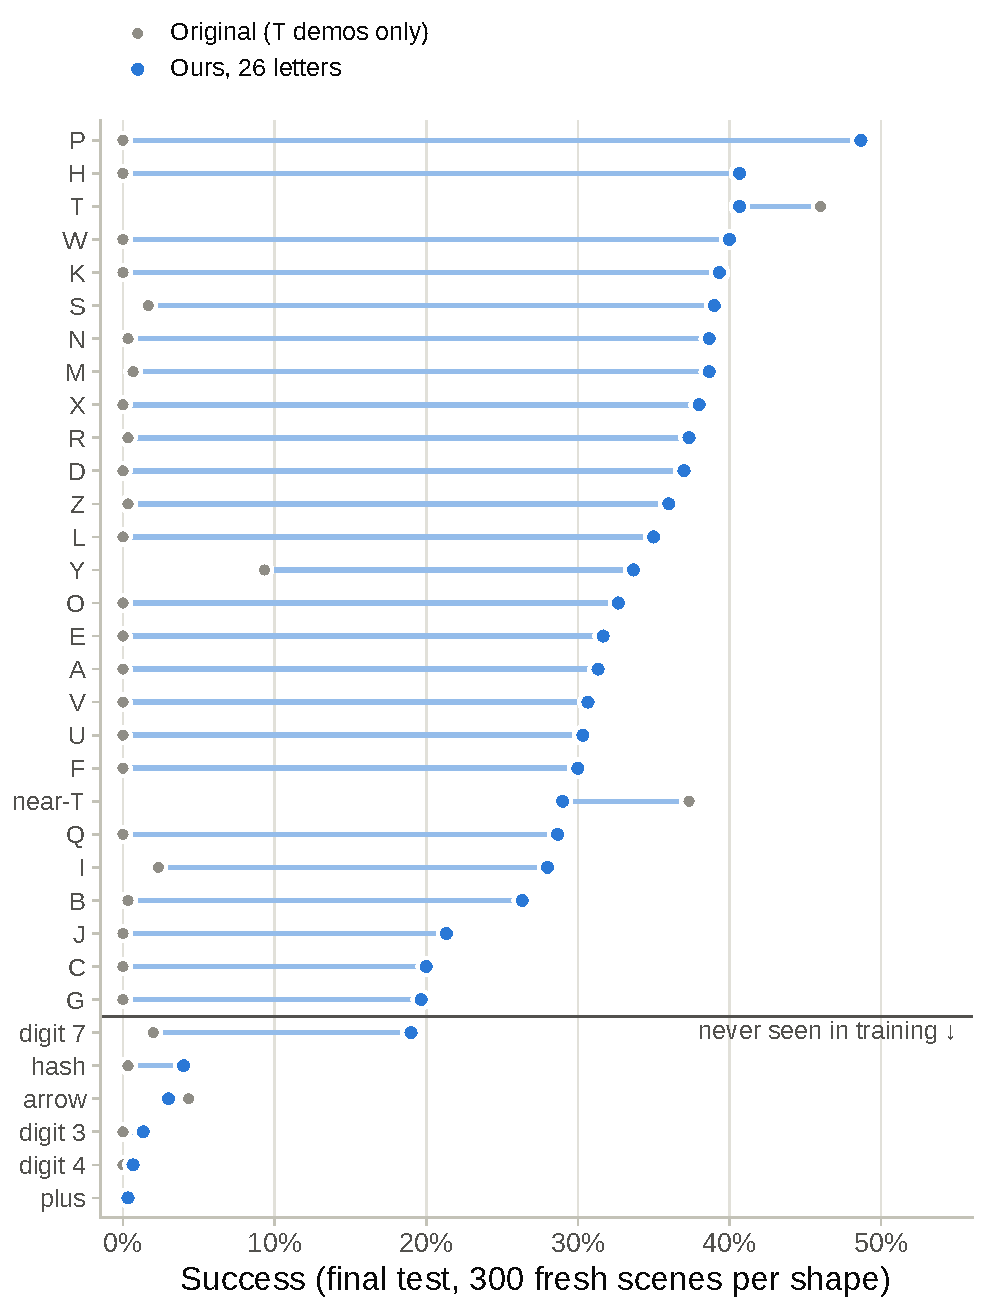
\includegraphics[width=\columnwidth]{../figures/final_dumbbell.pdf}
  \caption{Per-shape success, original $\rightarrow$ 27-shape student (96~px), final test, 300 scenes per shape.
  Held-out shapes are listed separately. \todo{regenerate at column size; full table in Table~\ref{tab:pershape}}}
  \label{fig:dumbbell}
\end{figure}

\paragraph{Earlier stages.}
On five shapes, correction round 4 raised average success from 18.5\% to 32.2\% on 1000 fresh scenes per letter, and
round 7 from 18.6\% to 34.2\% on another pool, with Y, D and L going from 0--10\% to 29--39\%. % D046, D047
On ten shapes (Table~\ref{tab:ten}), average success rose from 9.1\% to 34.3\% (96~px) and 38.2\% (192~px) on 1000
fresh scenes per shape, with T unchanged (42.2\% to 42.9\%, $+0.7$ $[-3.6, +5.0]$). % D049, D050
Average success stayed near 34\% as the shape set grew from 5 to 10 to 27.
\todo{optional: Fig. final\_stage\_progression}

\begin{table*}[t]
  \centering
  \caption{Ten-shape stage: success (\%) on 1000 fresh scenes per shape, paired by scene; change against the
  original in points with 95\% intervals.}
  \label{tab:ten}
  \begin{adjustbox}{max width=\textwidth}
  % Generated by presentation/scripts/make_figures.py from presentation/data/*.csv. Needs \usepackage{booktabs}.

\begin{tabular}{lrrrrr}
\toprule
Shape & Original & 96 px & Change & 192 px & Change \\
\midrule
T & 42.2 & 42.9 & +0.7 [$-$3.6, +5.0] & 44.5 & +2.3 [$-$2.1, +6.7] \\
near-T & 39.8 & 32.0 & $-$7.8 [$-$12.0, $-$3.6] & 36.0 & $-$3.8 [$-$8.0, +0.4] \\
Y & 8.4 & 39.4 & +31.0 [+27.5, +34.5] & 39.0 & +30.6 [+27.1, +34.1] \\
D & 0.1 & 42.5 & +42.4 [+39.3, +45.5] & 45.7 & +45.6 [+42.5, +48.7] \\
L & 0.0 & 34.7 & +34.7 [+31.7, +37.7] & 37.8 & +37.8 [+34.8, +40.8] \\
E & 0.0 & 26.7 & +26.7 [+24.0, +29.4] & 30.4 & +30.4 [+27.5, +33.3] \\
F & 0.5 & 26.1 & +25.6 [+22.9, +28.3] & 33.1 & +32.6 [+29.7, +35.5] \\
J & 0.0 & 23.8 & +23.8 [+21.2, +26.4] & 24.5 & +24.5 [+21.8, +27.2] \\
P & 0.4 & 47.3 & +46.9 [+43.8, +50.0] & 58.1 & +57.7 [+54.6, +60.8] \\
U & 0.0 & 27.4 & +27.4 [+24.6, +30.2] & 32.5 & +32.5 [+29.6, +35.4] \\
\midrule
\textbf{All 10} & 9.1 & 34.3 & +25.1 [+24.1, +26.2] & 38.2 & +29.0 [+27.9, +30.1] \\
\bottomrule
\end{tabular}
% Success %, final test, 1000 fresh scenes per shape, paired by scene; change in points with 95% interval.

  \end{adjustbox}
\end{table*}

\paragraph{Held-out shapes.}
On the six held-out shapes, success rises with the number of training shapes: 1.2\% (original, trained on T), 2.8\%
(ten shapes), 4.7\% and 5.9\% (27 shapes, 96 and 192~px), and mean final coverage from 0.43 to 0.56--0.58
(Fig.~\ref{fig:heldout}). Most of the gain is on digit 7 (2.0\% to 19.0--23.0\%), which shares strokes with trained
letters; digit 3, digit 4, plus and arrow stay at or below 3\%. Before the 27-shape stage, the ten-shape students
reached 6.6\% (96~px) and 10.6\% (192~px) on the 17 capitals they had not trained on, against 0.2\% for the original
(Table~\ref{tab:unseen}). % D051, D052
This is modest transfer; the main result is adaptation with machine-generated practice on the target shapes.

\begin{figure}[t]
  \centering
  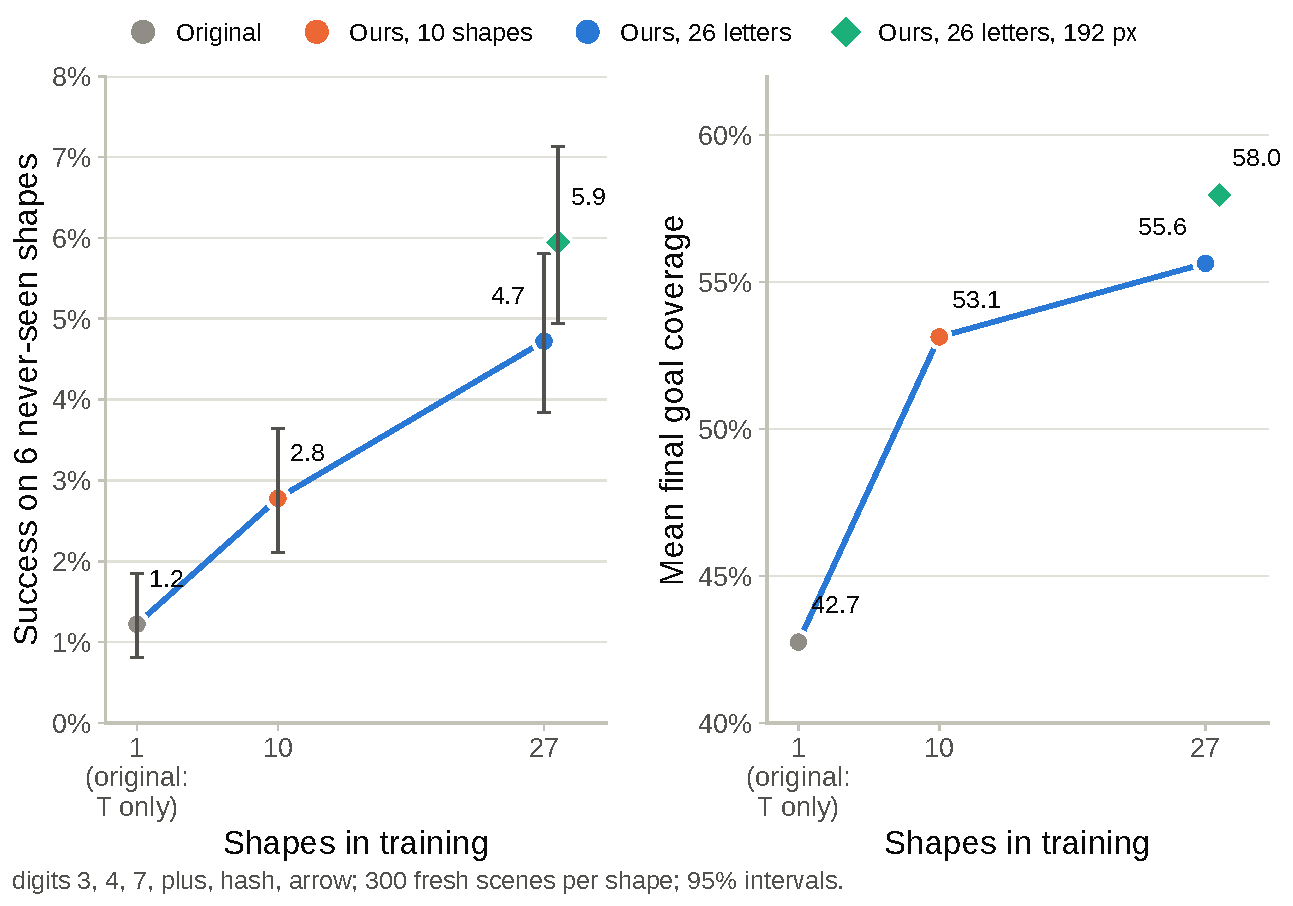
\includegraphics[width=\columnwidth]{../figures/heldout_scaling.pdf}
  \caption{Held-out shapes: success and final coverage against the number of training shapes (1, 10, 27).}
  \label{fig:heldout}
\end{figure}

\paragraph{Where the remaining failures are.}
Most failed episodes end close to the goal. Over the 27 trained shapes, mean final coverage is 0.82 and mean peak
coverage 0.91, but success needs more than 0.95 (Fig.~\ref{fig:nearmiss}). Success allows only 1.3--2.7 simulator
pixels of position error, which is 0.24--0.51 of a 96~px camera pixel (Fig.~\ref{fig:zoom}). The 192~px camera helps on
ten shapes ($+3.9$ points $[+2.6, +5.2]$ over 10,000 paired scenes) but not on 27 shapes (33.8\% against 33.4\%,
$+0.3$ $[-1.1, +1.8]$; Fig.~\ref{fig:192}), so resolution is not the whole story. \todo{one sentence each on
coverage\_cdf and the share of episodes that peak between 90\% and 95\%}
% The 27-shape 192-vs-96 interval was computed from data/final_tests_episodes.csv (D051, paired by scene);
% check it against figures/analysis_192_vs_96 before submission.

\begin{figure}[t]
  \centering
  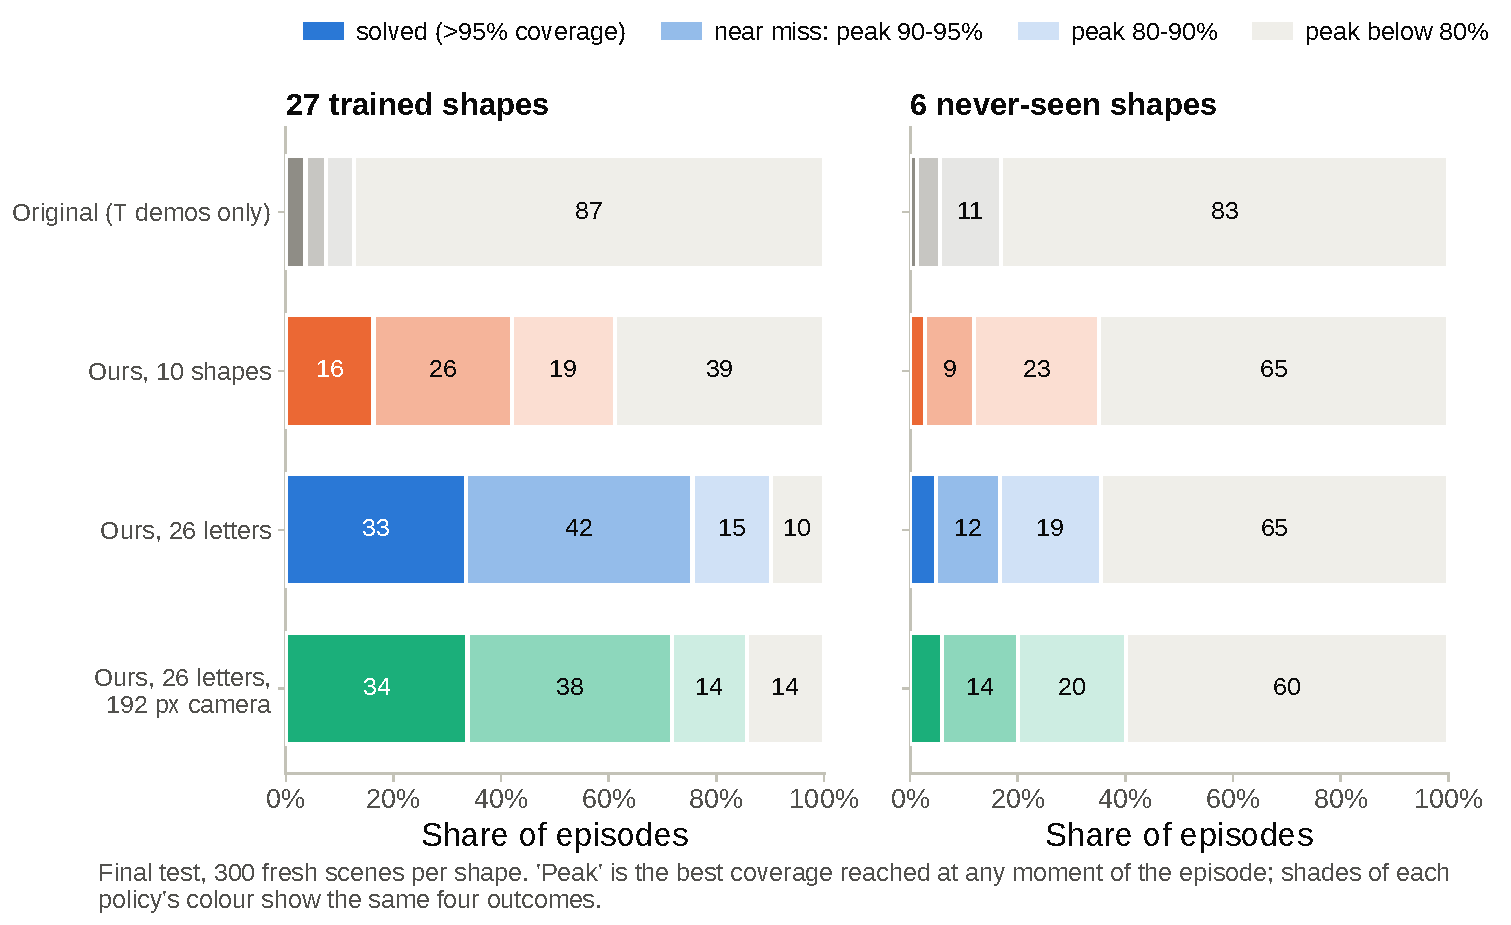
\includegraphics[width=\columnwidth]{../figures/coverage_near_misses.pdf}
  \caption{Episode outcomes on the final test: solved, near miss (peak coverage 90--95\%), peak 80--90\%, and lower,
  for trained and held-out shapes.}
  \label{fig:nearmiss}
\end{figure}

\begin{figure}[t]
  \centering
  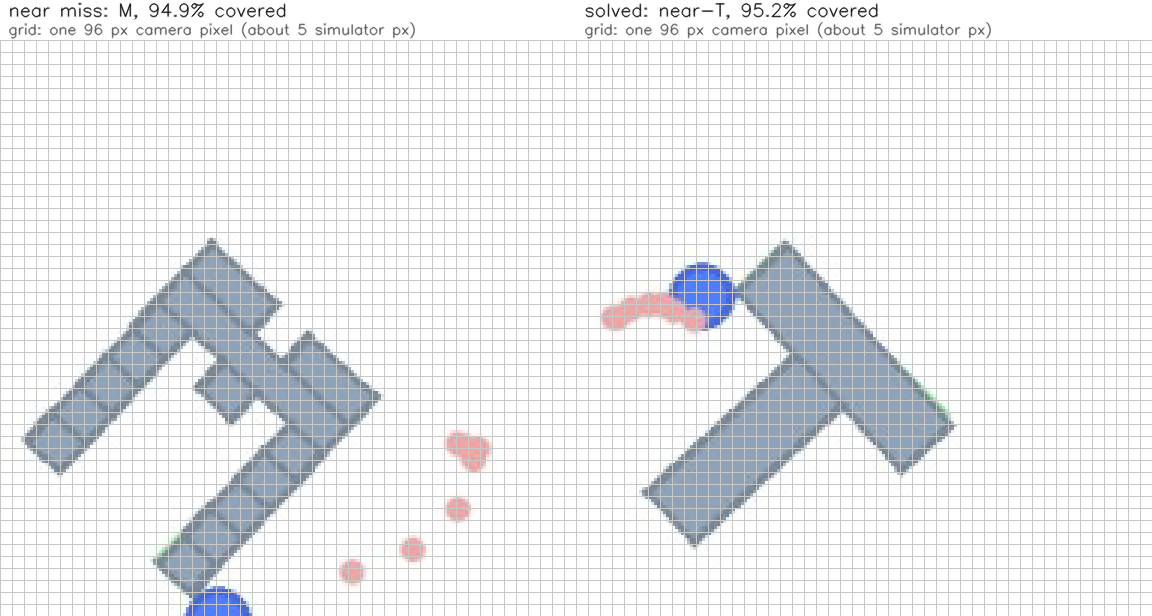
\includegraphics[width=\columnwidth]{../images/last_mile/near_miss_vs_solved_zoom.png}
  \caption{A near miss (M, 94.9\% covered) next to a success (near-T, 95.2\%). Grid: one 96~px camera pixel, about 5
  simulator pixels.}
  \label{fig:zoom}
\end{figure}

\paragraph{Ablations and design choices.}
\label{sec:ablations}
Table~\ref{tab:labels} lists matched A/B tests from the ten-shape stage (validation, 100 scenes per shape). Only the
label change is clearly beyond test noise (about $\pm30$ of 1000): intended-plan labels gave 129 successes against 77
for executed-push labels. A sharper camera (111 to 129), twice the teacher data (104 to 111) and a four times larger
action network trained from scratch (138 to 146) gave smaller, uncertain gains. Executing more of each 16-step plan is
much worse: 12 steps give 18.6\% and 15 steps 12.2\% against 34.8\% with the trained 8 (Fig.~\ref{fig:steps}); even the
teacher keeps only 78\% of its successes when it must commit to 8 pushes. % D048, D056
\todo{move the camera and network rows into the text if the table is cut}

\begin{table}[t]
  \centering
  \caption{Matched A/B tests, ten-shape stage: validation success (\%), 100 scenes $\times$ 10 shapes, official recipe,
  30k steps (network-size row: both from scratch, 50k steps).}
  \label{tab:labels}
  \begin{adjustbox}{max width=\columnwidth}
  % Generated by presentation/scripts/make_figures.py from presentation/data/*.csv. Needs \usepackage{booktabs}.

\begin{tabular}{lrr}
\toprule
Change & Without & With \\
\midrule
Copy the teacher's intended plan instead of its executed pushes & 7.7 & 12.9 \\
Camera 192 px instead of 96 px & 11.1 & 12.9 \\
All teacher demonstrations instead of half & 10.4 & 11.1 \\
Action network 990M instead of 251M parameters (from scratch) & 13.8 & 14.6 \\
\bottomrule
\end{tabular}
% Validation success %, 100 scenes x 10 shapes; typed in from docs/LEARNING_FINDINGS.md section 7.

  \end{adjustbox}
\end{table}

\begin{figure}[t]
  \centering
  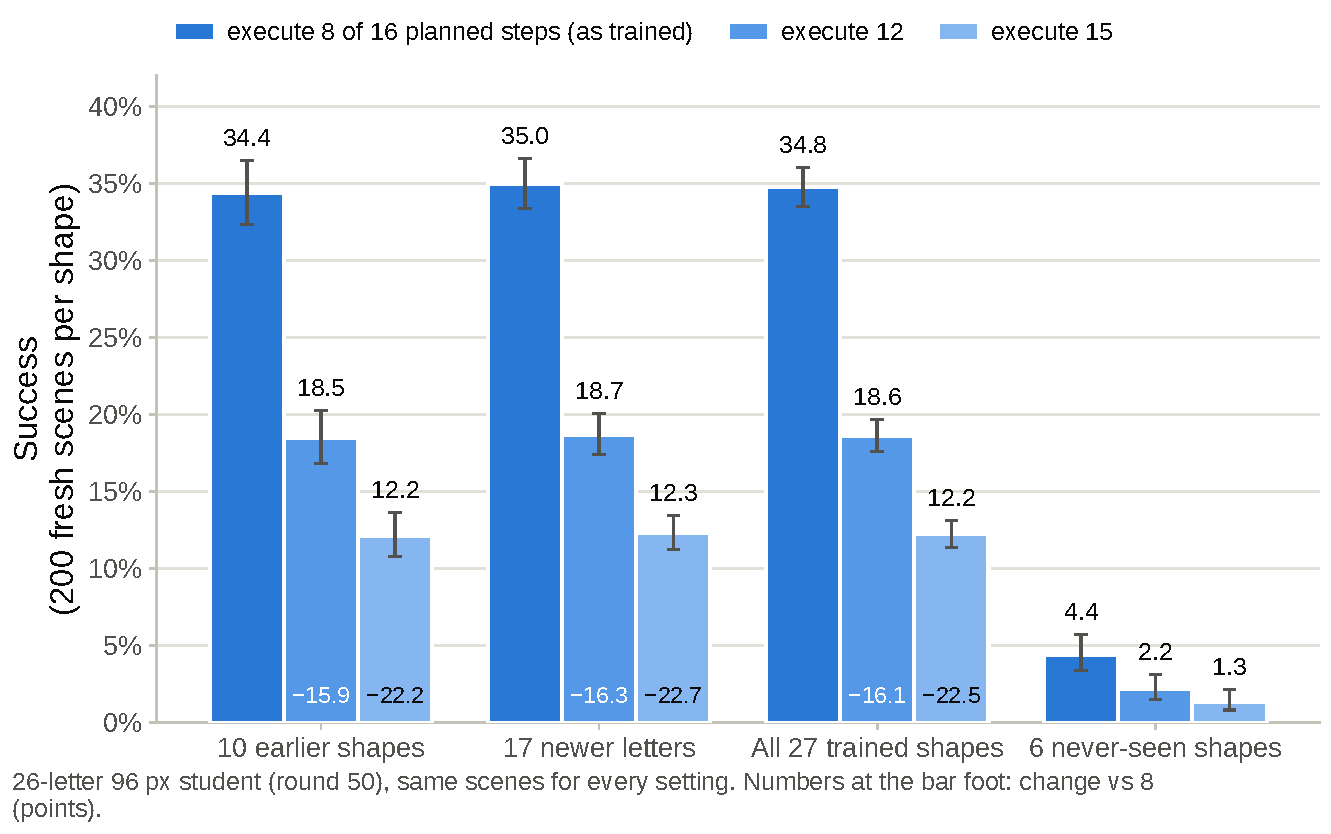
\includegraphics[width=\columnwidth]{../figures/analysis_steps_executed.pdf}
  \caption{Steps executed per 16-step plan before planning again (round-50 student, 200 fresh scenes per shape,
  paired). The trained setting (8) is best on every group. Table~\ref{tab:steps} gives the numbers.}
  \label{fig:steps}
\end{figure}

\begin{figure}[t]
  \centering
  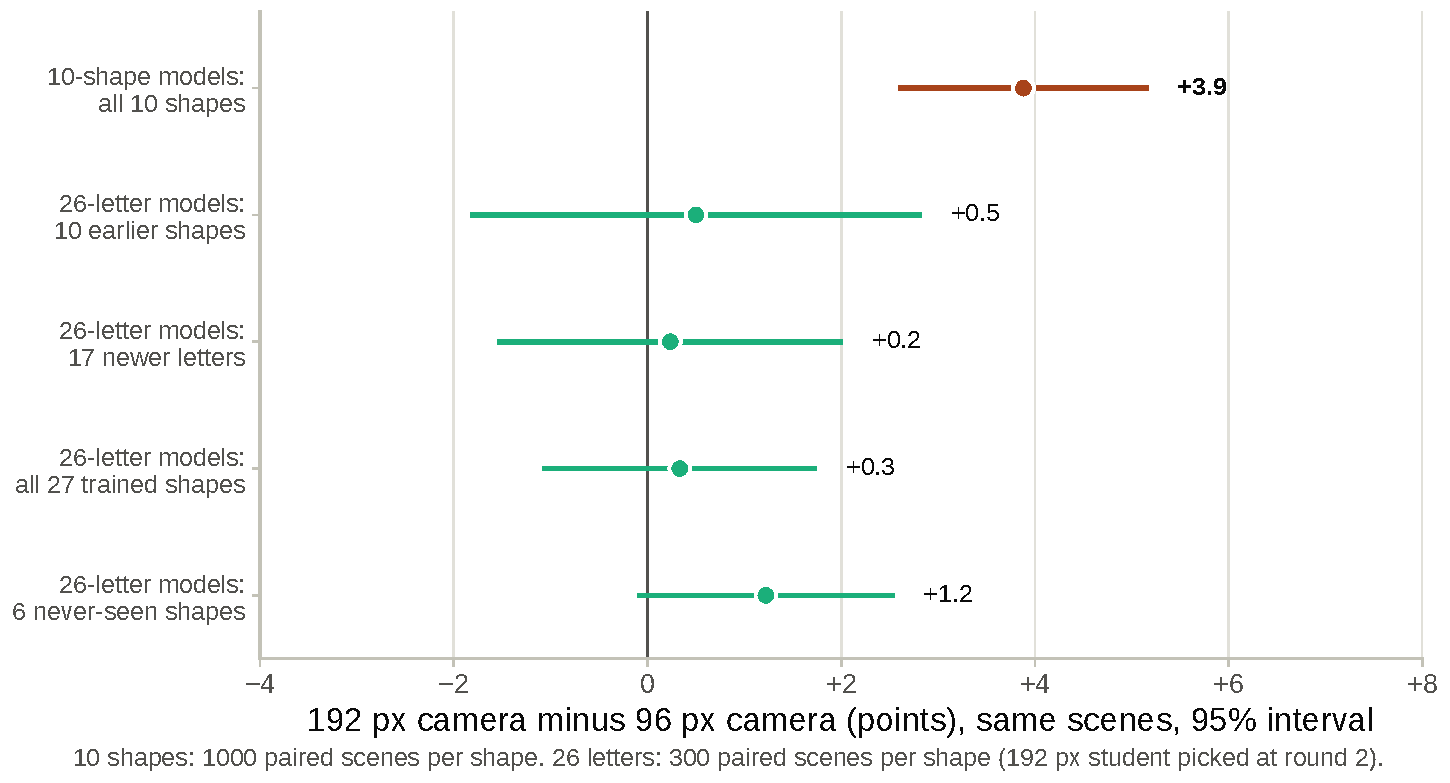
\includegraphics[width=\columnwidth]{../figures/analysis_192_vs_96.pdf}
  \caption{192~px minus 96~px camera, paired by scene, for the ten-shape and 27-shape students.}
  \label{fig:192}
\end{figure}

\begin{table}[t]
  \centering
  \caption{Round 50 against the pre-registered round 44 (96~px): success (\%) on 200 fresh scenes per shape, paired by
  scene.}
  \label{tab:r50}
  \begin{adjustbox}{max width=\columnwidth}
  % Generated by presentation/scripts/make_figures.py from presentation/data/*.csv. Needs \usepackage{booktabs}.

\begin{tabular}{lrrr}
\toprule
Shapes & Round 44 & Round 50 & Change \\
\midrule
10 earlier shapes & 34.0 & 34.4 & +0.4 [$-$2.5, +3.3] \\
17 newer letters & 32.3 & 35.0 & +2.7 [+0.6, +4.9] \\
All 27 trained shapes & 32.9 & 34.8 & +1.9 [+0.1, +3.6] \\
6 never-seen shapes & 4.8 & 4.4 & $-$0.4 [$-$2.0, +1.2] \\
\bottomrule
\end{tabular}
% 27-shape 96 px student; separate fresh pool (D054), 200 scenes per shape, paired by scene; not comparable with the D051 final-test numbers.

  \end{adjustbox}
\end{table}

\paragraph{T and near-T.}
Adapting to 27 shapes costs some T and near-T success. In the final test T fell from 46.0\% to 40.7\% at 96~px
($-5.3$ $[-13.5, +2.9]$, interval includes zero) and to 38.3\% at 192~px ($-7.7$ $[-15.1, -0.2]$); near-T fell from
37.3\% to 29.0\% ($-8.3$ $[-15.9, -0.7]$) and 32.3\% ($-5.0$ $[-12.2, +2.2]$) (Fig.~\ref{fig:ttradeoff}). The ten-shape
student showed no measurable T change on 1000 scenes per shape but lost near-T ($-7.8$ $[-12.0, -3.6]$), and round 50 scored 44.0\%
on T against 38.0\% for round 44 on the same 200 scenes. The students push T closer to the goal on average (mean final
coverage on T 0.73 to 0.86 in the final test) but finish it less often. % D049, D051, D054
\todo{decide whether to present the T/near-T trade-off as a limitation, a result, or both}

\begin{figure}[t]
  \centering
  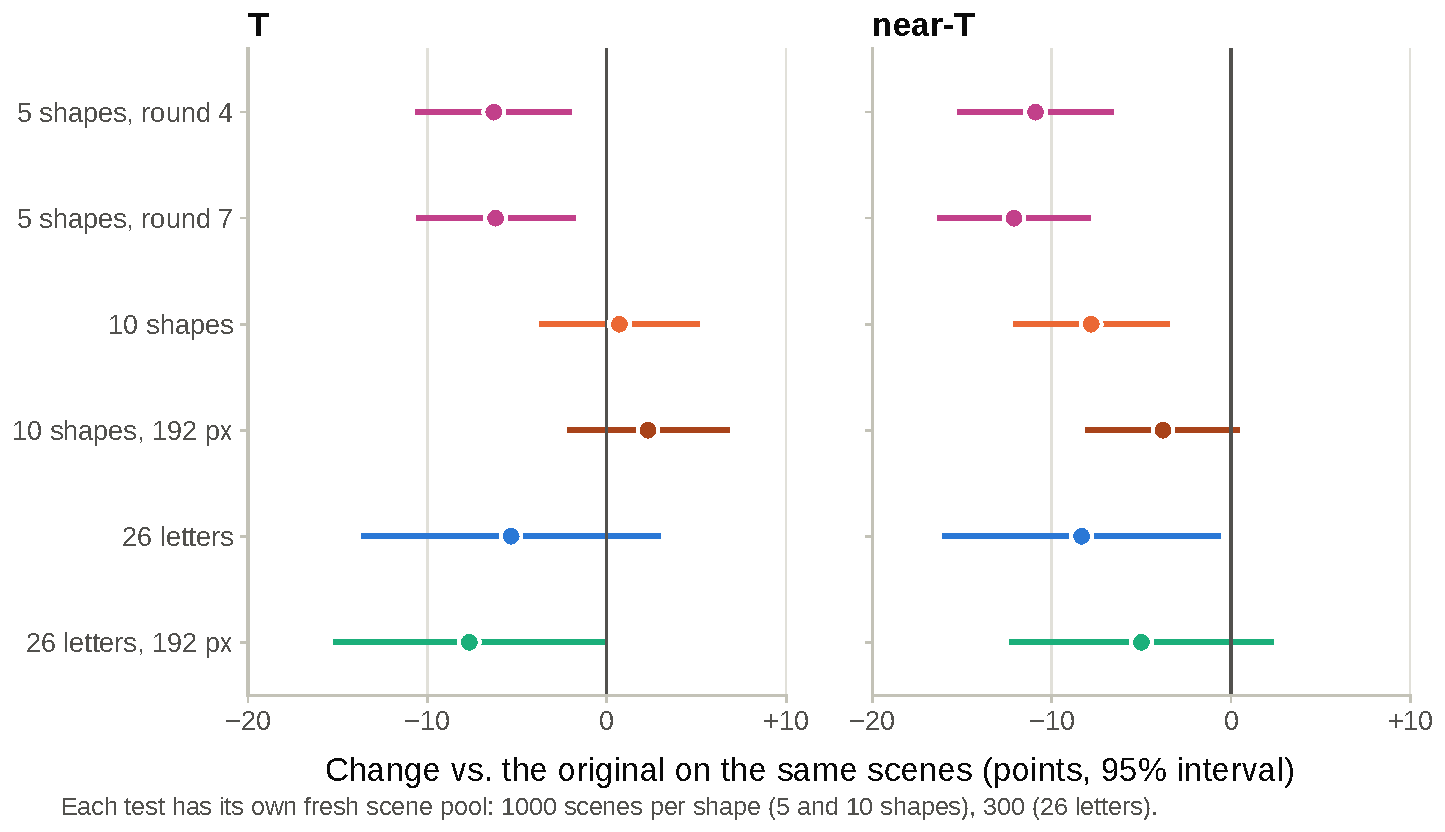
\includegraphics[width=\columnwidth]{../figures/analysis_t_tradeoff_diff.pdf}
  \caption{T and near-T: paired change against the original with 95\% intervals for each student.}
  \label{fig:ttradeoff}
\end{figure}

% =====================================================================================================================
\section{Limitations and disclosure}
\label{sec:limits}

\paragraph{Limitations.}
All results are in simulation; we have not tested a real robot. Success is about one in three on the trained shapes,
far below the teacher (78\% on ten shapes), and the gap is mostly in the last few simulator pixels of alignment. Transfer to
shapes never trained on is small (4.7--5.9\%), so the method is adaptation with target-shape practice data, not
zero-shot generalization. T and near-T lose some success. The validation curves are noisy enough that we cannot tell
apart most late correction rounds. \todo{compute cost: single H100 NVL and A100 GPUs, several 3-day jobs; about 54k
training steps per correction round; total GPU hours}

\paragraph{Disclosure.}
The teacher reads the simulator's exact block and pusher state (with 1~px / 1$^\circ$ added noise); the tested policies
see only camera frames and the pusher position. The planner's push candidates are a hand-designed geometric exploration
prior, and its reward uses privileged geometry (letter rectangles, goal pose, coverage); the world model's pusher
dynamics and contact geometry are copied from the simulator, and only the block's motion in contact is learned. No new
human demonstrations, teleoperation or success labels were collected, but every student reuses the 206 human T
demonstrations that the released checkpoint was trained on, next to the machine-generated data. Each setting was
trained once (one run, one seed), so we report no training-seed variability. The 50 validation scenes per shape were
reused across rounds to pick checkpoints, which biases validation numbers upward (for example, the 192~px pick led on
validation, 511 against 470 of 1350, but not on fresh scenes; Fig.~\ref{fig:app-selection}). Every final test used a
fresh seed pool that had never been used before, fixed together with the candidate and the analysis before the run;
the one exception is the steps-executed test, which reused the round-50 scenes and was fixed to need a confirmation on
unused scenes had any setting beaten the trained one. % D056
The 192~px students use a sharper camera than the original policy and are reported as a sensor change.
\todo{add the earlier pre-registered blend tests (three failed, one passed and replicated) to the disclosure or
appendix so all looks at test data are listed}

% =====================================================================================================================
\section{Conclusion}
\label{sec:conclusion}

A camera Diffusion Policy that knew only the T now pushes all 26 capital letters and near-T, with success over the 27
trained shapes rising from 3.7\% to 33--35\% on fresh scenes, without any new human demonstrations. The levers that
mattered were a world-model planner as a privileged teacher, labels that use the teacher's intended plans, correction
rounds on the student's own states, and enough training per shape. RL fine-tuning in the simulator did not work here
because its training signal was mostly noise. The open problem is final alignment: blocks usually end close to the goal
but miss the 95\% coverage threshold. \todo{next steps: last-mile corrections, finer camera or state estimate, real
robot; link to code and model if allowed}

% =====================================================================================================================
\bibliographystyle{plainnat}
% Compiled inside paper/ -> refs.bib; compiled from the presentation/ root through a proxy file (README.md, Option B)
% -> BibTeX runs in the root and needs paper/refs.bib.
\IfFileExists{paper/refs.bib}{\bibliography{paper/refs}}{\bibliography{refs}}

% =====================================================================================================================
\appendix
\onecolumn
\section{Additional results}
\label{sec:appendix}
\todo{trim this appendix to what the course allows; every item below exists as a file}

\begin{table}[h]
  \centering
  \caption{Per-shape success (\%), final test, 300 fresh scenes per shape. Left block: the ten earlier shapes then the
  first seven newer letters; right block: the remaining newer letters, then the six held-out shapes (digit 3 to
  arrow). Orig.\ = original; 10 sh.\ = ten-shape student; 26 l.\ = 27-shape student, 96~px; 192 px = 27-shape student,
  192~px.}
  \label{tab:pershape}
  \begin{adjustbox}{max width=\textwidth}
  % Generated by presentation/scripts/make_figures.py from presentation/data/*.csv. Needs \usepackage{booktabs}.

\begin{tabular}{lrrrr@{\hspace{1.5em}}lrrrr}
\toprule
Shape & Orig. & 10 sh. & 96 px & 192 px & Shape & Orig. & 10 sh. & 96 px & 192 px \\
\midrule
T & 46.0 & 42.7 & 40.7 & 38.3 & M & 0.7 & 1.7 & 38.7 & 37.7 \\
near-T & 37.3 & 32.0 & 29.0 & 32.3 & N & 0.3 & 0.3 & 38.7 & 41.7 \\
Y & 9.3 & 33.7 & 33.7 & 33.7 & O & 0.0 & 17.0 & 32.7 & 39.0 \\
D & 0.0 & 38.7 & 37.0 & 44.0 & Q & 0.0 & 6.3 & 28.7 & 22.0 \\
L & 0.0 & 30.3 & 35.0 & 34.0 & R & 0.3 & 10.7 & 37.3 & 28.0 \\
E & 0.0 & 23.3 & 31.7 & 28.0 & S & 1.7 & 3.3 & 39.0 & 33.7 \\
F & 0.0 & 28.3 & 30.0 & 29.3 & V & 0.0 & 5.0 & 30.7 & 27.3 \\
J & 0.0 & 21.3 & 21.3 & 19.0 & W & 0.0 & 12.0 & 40.0 & 39.0 \\
P & 0.0 & 46.7 & 48.7 & 51.3 & X & 0.0 & 2.3 & 38.0 & 36.7 \\
U & 0.0 & 33.3 & 30.3 & 32.3 & Z & 0.3 & 6.0 & 36.0 & 39.3 \\
A & 0.0 & 2.7 & 31.3 & 25.0 & digit 3 & 0.0 & 0.0 & 1.3 & 1.7 \\
B & 0.3 & 20.0 & 26.3 & 39.7 & digit 4 & 0.0 & 0.7 & 0.7 & 0.7 \\
C & 0.0 & 3.7 & 20.0 & 17.7 & digit 7 & 2.0 & 10.3 & 19.0 & 23.0 \\
G & 0.0 & 4.0 & 19.7 & 20.3 & plus & 0.7 & 1.3 & 0.3 & 0.3 \\
H & 0.0 & 4.3 & 40.7 & 45.7 & hash & 0.3 & 2.0 & 4.0 & 7.3 \\
I & 2.3 & 5.7 & 28.0 & 35.3 & arrow & 4.3 & 2.3 & 3.0 & 2.7 \\
K & 0.0 & 4.3 & 39.3 & 41.0 &  & & & &  \\
\bottomrule
\end{tabular}
% Success %, final test (D051), 300 fresh scenes per shape; 96 px and 192 px = the 27-shape students of rounds 44 and 2. Order: 10 earlier shapes, 17 newer letters, 6 never-seen shapes (digit 3 ... arrow).

  \end{adjustbox}
\end{table}

\begin{table}[h]
  \centering
  \caption{Steps executed per plan (round-50 student, 200 fresh scenes per shape, paired by scene).}
  \label{tab:steps}
  \begin{adjustbox}{max width=\textwidth}
  % Generated by presentation/scripts/make_figures.py from presentation/data/*.csv. Needs \usepackage{booktabs}.

\begin{tabular}{lrrrrr}
\toprule
Shapes & Execute 8 & Execute 12 & Change & Execute 15 & Change \\
\midrule
10 earlier shapes & 34.4 & 18.5 & $-$15.9 [$-$17.5, $-$14.3] & 12.2 & $-$22.2 [$-$24.1, $-$20.4] \\
17 newer letters & 35.0 & 18.7 & $-$16.3 [$-$17.5, $-$15.1] & 12.3 & $-$22.7 [$-$24.1, $-$21.3] \\
All 27 trained shapes & 34.8 & 18.6 & $-$16.1 [$-$17.1, $-$15.2] & 12.2 & $-$22.5 [$-$23.7, $-$21.4] \\
6 never-seen shapes & 4.4 & 2.2 & $-$2.2 [$-$3.1, $-$1.4] & 1.3 & $-$3.1 [$-$4.1, $-$2.1] \\
\bottomrule
\end{tabular}
% Steps of each 16-step plan executed before re-planning; round-50 student, 200 fresh scenes per shape, paired by scene.

  \end{adjustbox}
\end{table}

\begin{table}[h]
  \centering
  \caption{Ten-shape students on the 17 capitals none of them trained on (200 fresh scenes per letter).}
  \label{tab:unseen}
  \begin{adjustbox}{max width=\textwidth}
  % Generated by presentation/scripts/make_figures.py from presentation/data/*.csv. Needs \usepackage{booktabs}.

\begin{tabular}{lrrr}
\toprule
Letter & Original & 10 shapes, 96 px & 10 shapes, 192 px \\
\midrule
A & 0.5 & 0.5 & 3.0 \\
B & 0.0 & 20.0 & 39.5 \\
C & 0.0 & 4.5 & 8.5 \\
G & 0.0 & 2.0 & 5.0 \\
H & 0.0 & 5.5 & 5.5 \\
I & 1.5 & 3.5 & 6.0 \\
K & 0.0 & 4.5 & 9.0 \\
M & 0.5 & 2.5 & 3.5 \\
N & 0.0 & 1.0 & 7.5 \\
O & 0.0 & 18.5 & 22.5 \\
Q & 0.0 & 7.0 & 13.5 \\
R & 0.0 & 11.5 & 15.0 \\
S & 1.0 & 4.0 & 4.0 \\
V & 0.0 & 6.0 & 9.0 \\
W & 0.0 & 13.5 & 19.5 \\
X & 0.5 & 3.5 & 1.5 \\
Z & 0.0 & 3.5 & 8.0 \\
\midrule
\textbf{All 17} & 0.2 & 6.6 & 10.6 \\
\bottomrule
\end{tabular}
% Success % of 10-shape students on the 17 capitals they never trained on; 200 fresh scenes per letter.

  \end{adjustbox}
\end{table}

\begin{figure}[h]
  \centering
  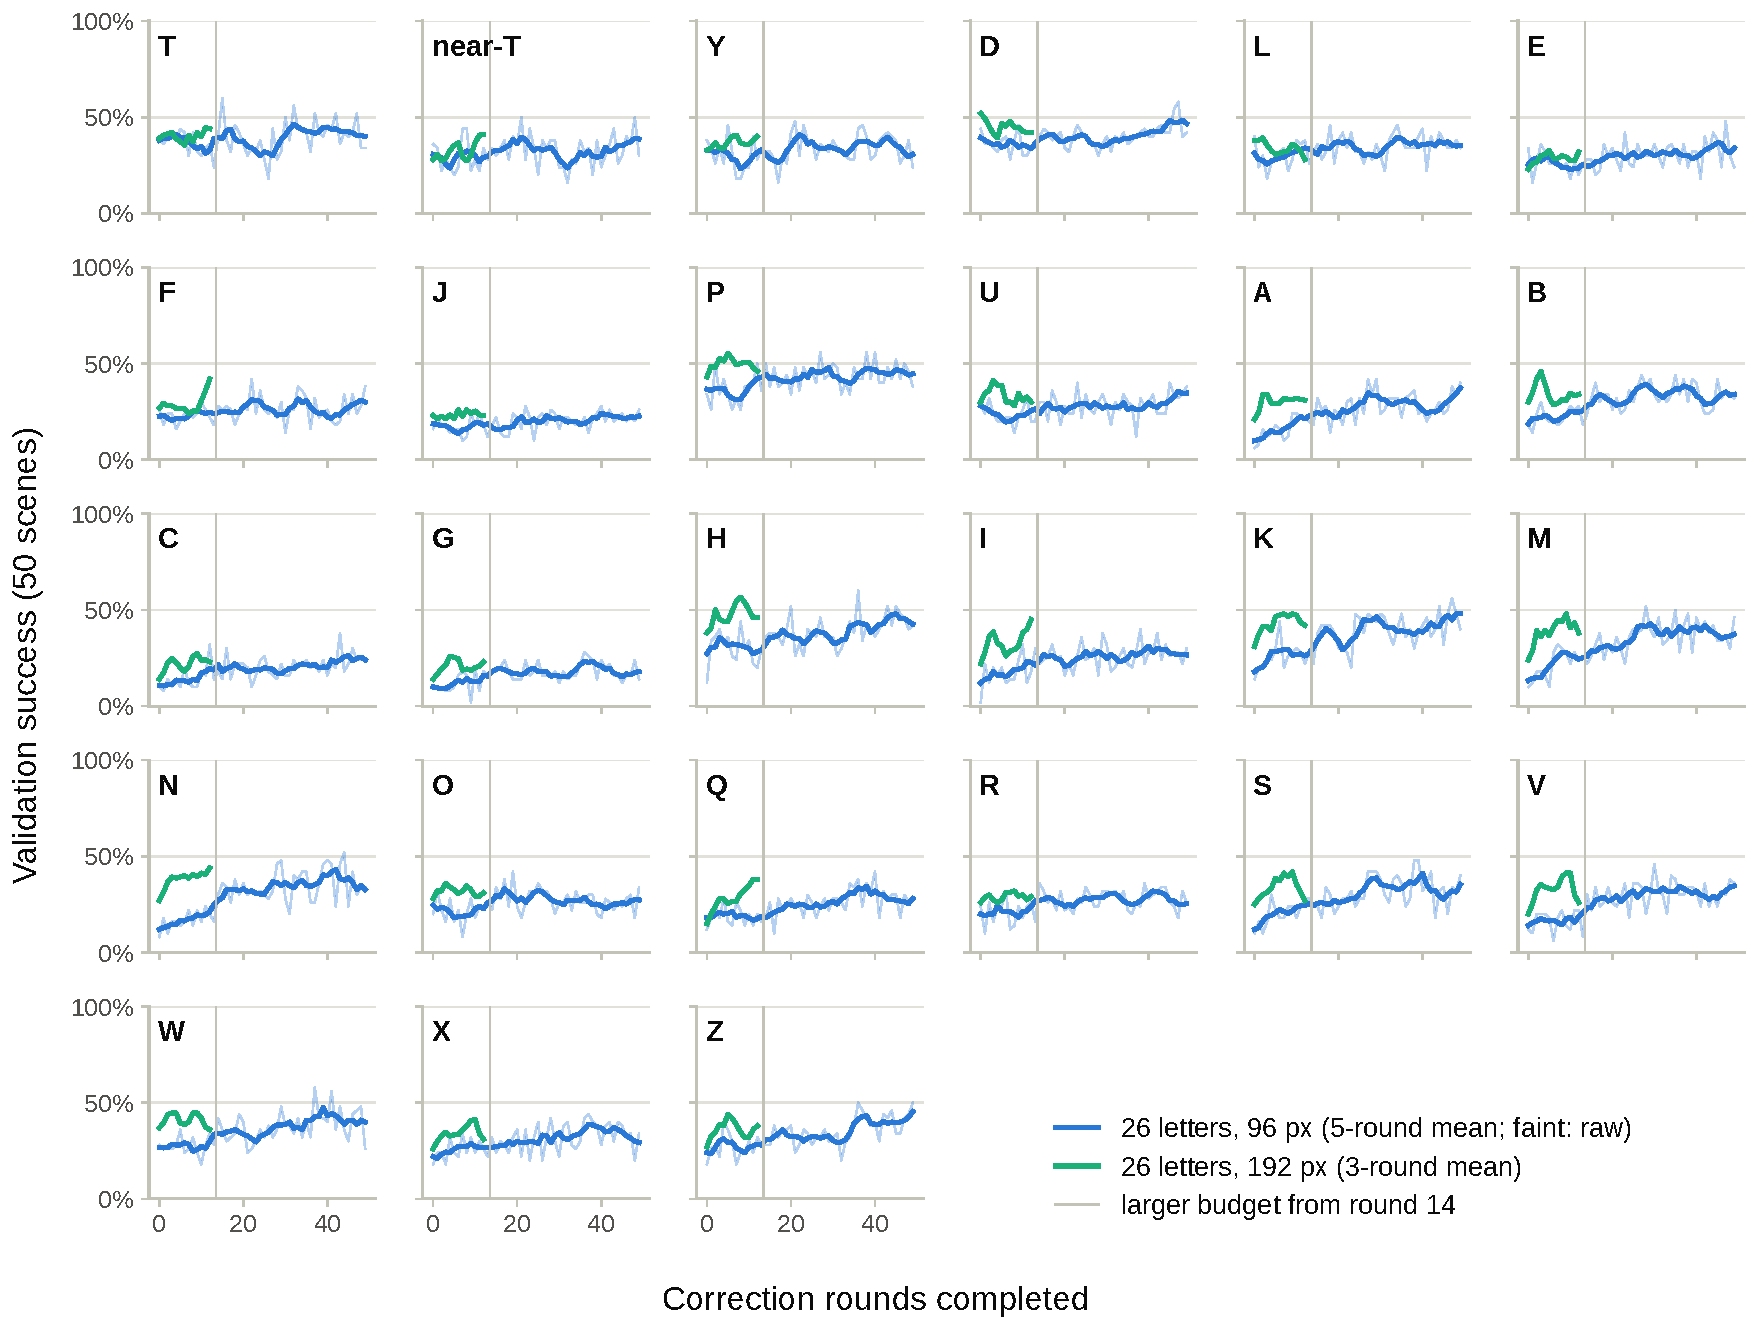
\includegraphics[width=0.9\textwidth]{../figures/curves_26letters_small_multiples.pdf}
  \caption{Validation success per shape over the 27-shape correction rounds (rolling means).}
  \label{fig:app-small-multiples}
\end{figure}

\begin{figure}[h]
  \centering
  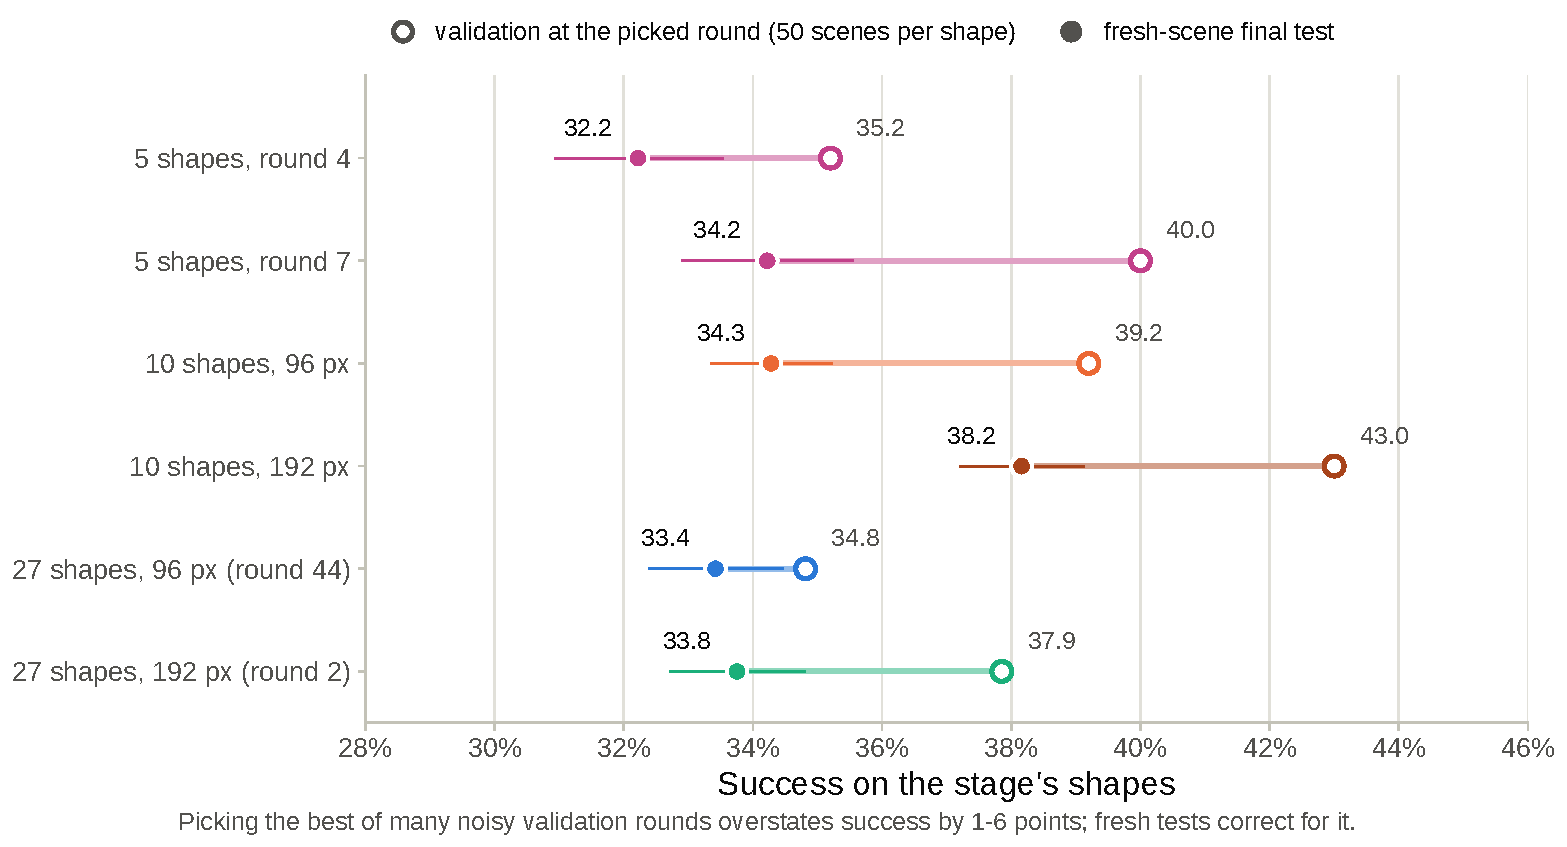
\includegraphics[width=0.48\textwidth]{../figures/analysis_selection_bias.pdf}\hfill
  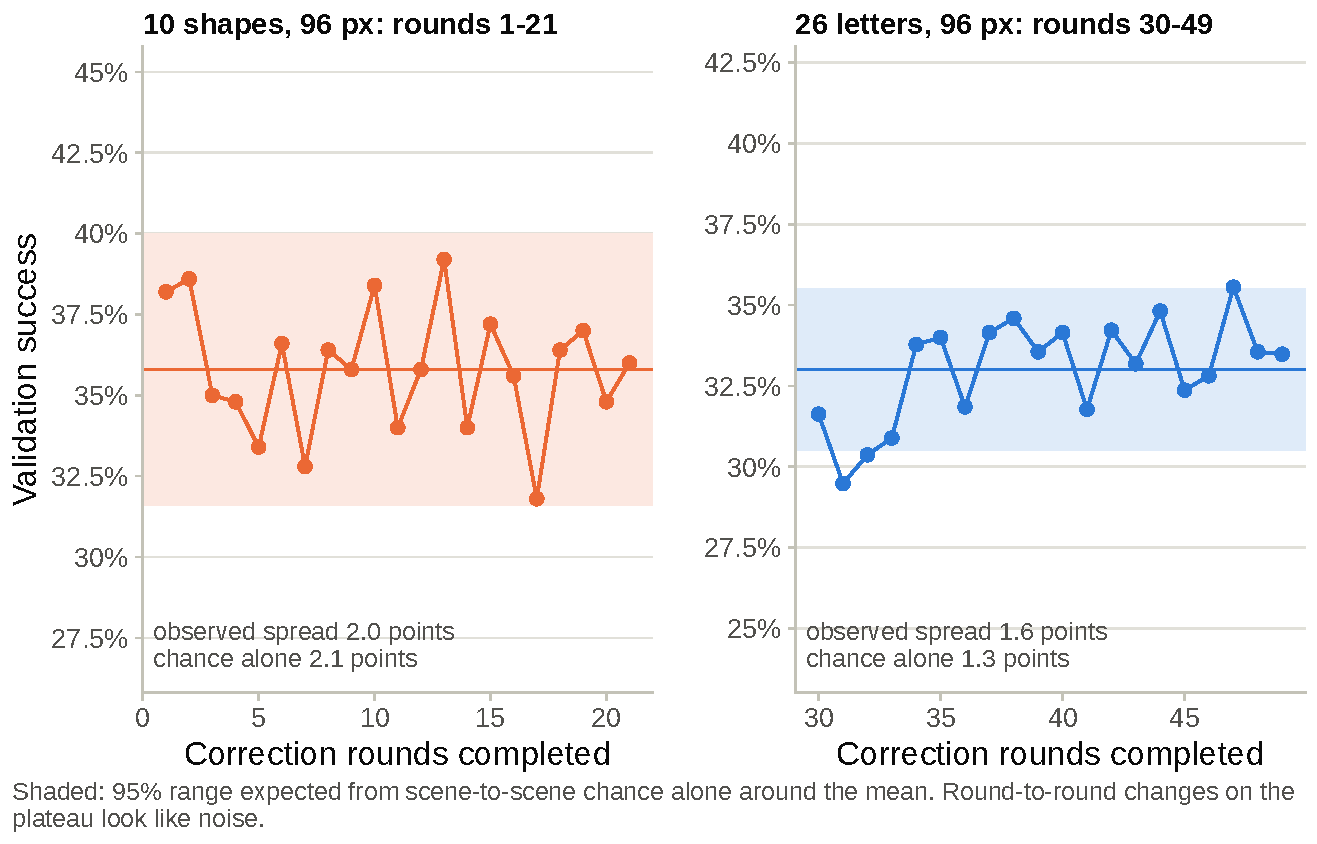
\includegraphics[width=0.48\textwidth]{../figures/analysis_plateau_noise.pdf}
  \caption{Left: validation success at the picked round against the fresh-scene test for every picked student
  (selection bias). Right: late validation rounds against the band expected from chance alone.}
  \label{fig:app-selection}
\end{figure}

\begin{figure}[h]
  \centering
  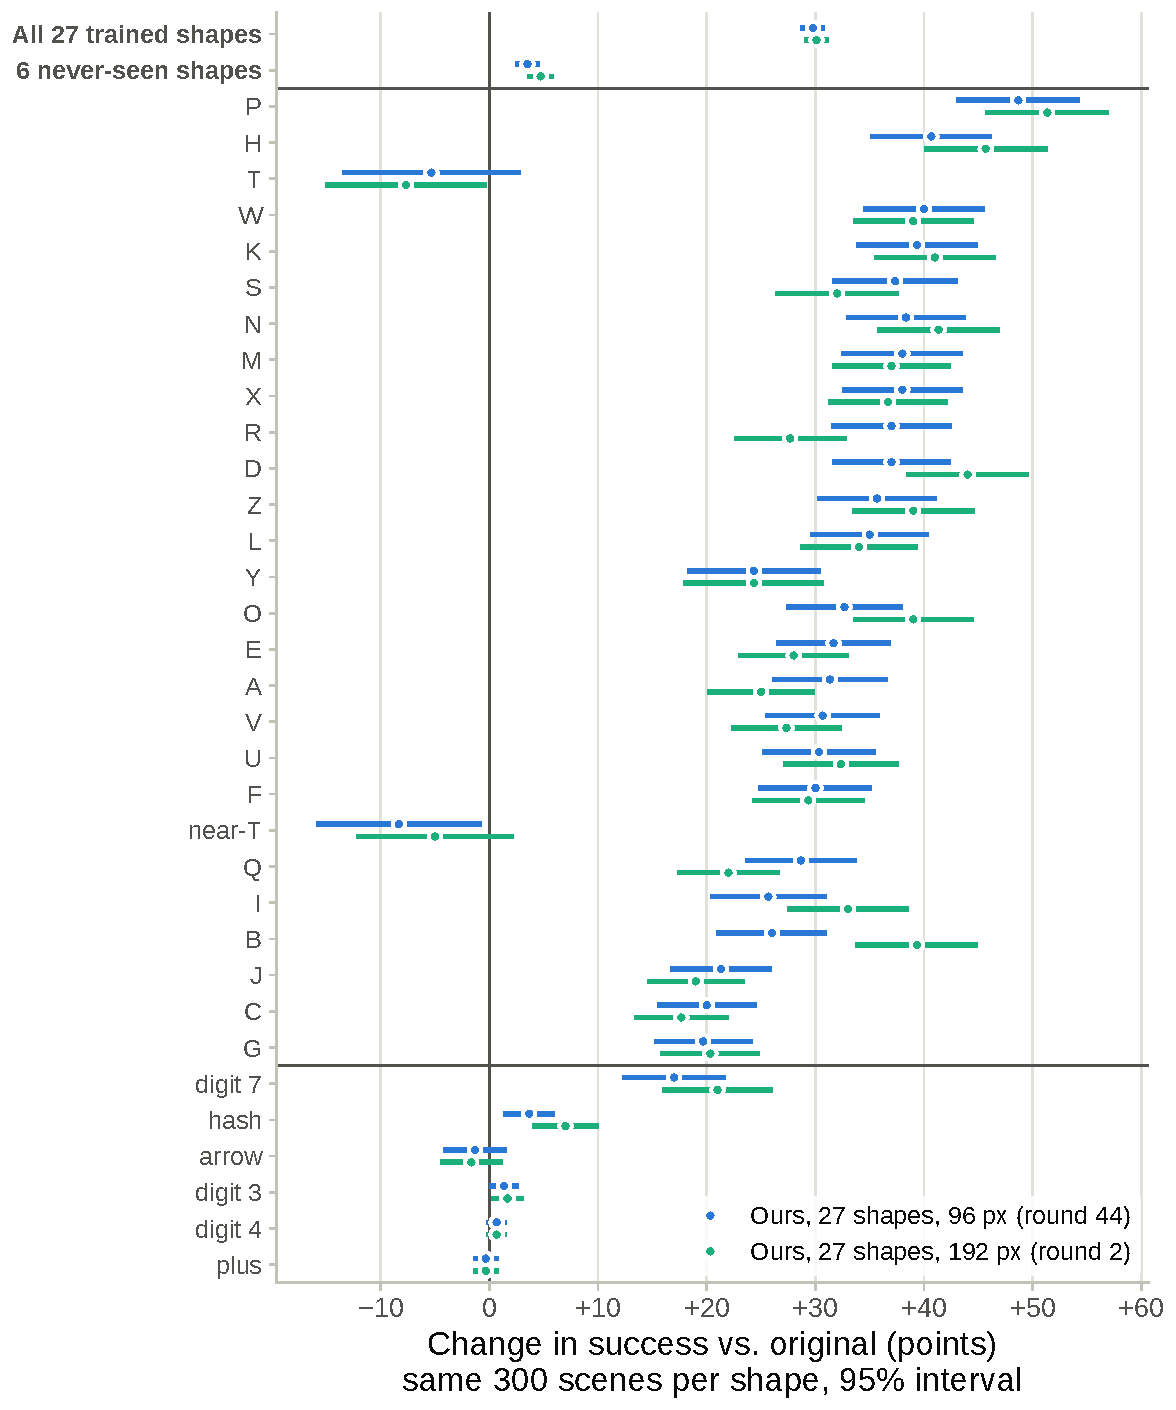
\includegraphics[width=0.48\textwidth]{../figures/final_forest_shapes.pdf}\hfill
  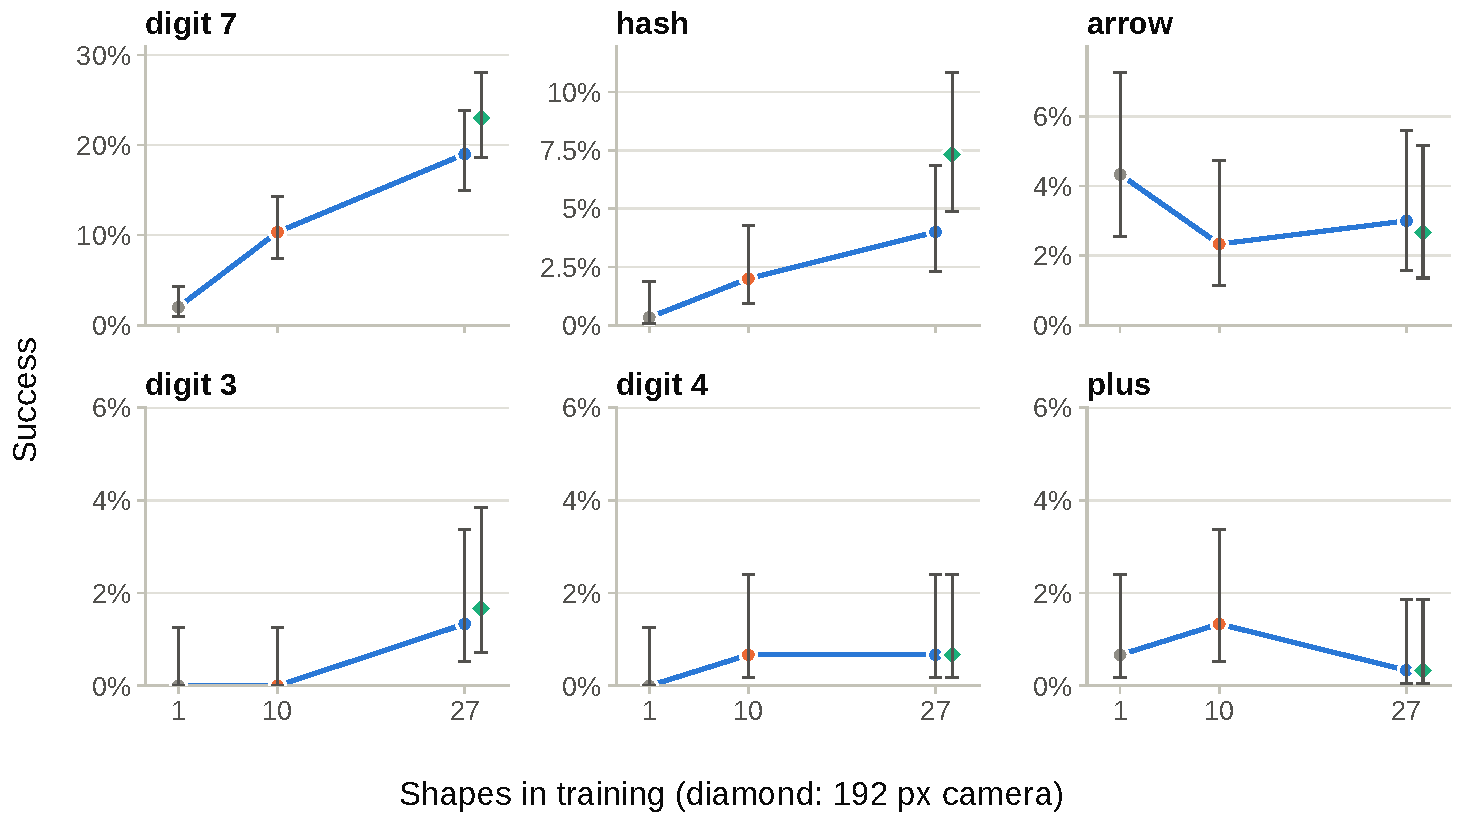
\includegraphics[width=0.48\textwidth]{../figures/heldout_scaling_per_shape.pdf}
  \caption{Left: paired change against the original for every shape (27-shape students). Right: each held-out shape
  against the number of training shapes.}
  \label{fig:app-forest}
\end{figure}

\begin{figure}[h]
  \centering
  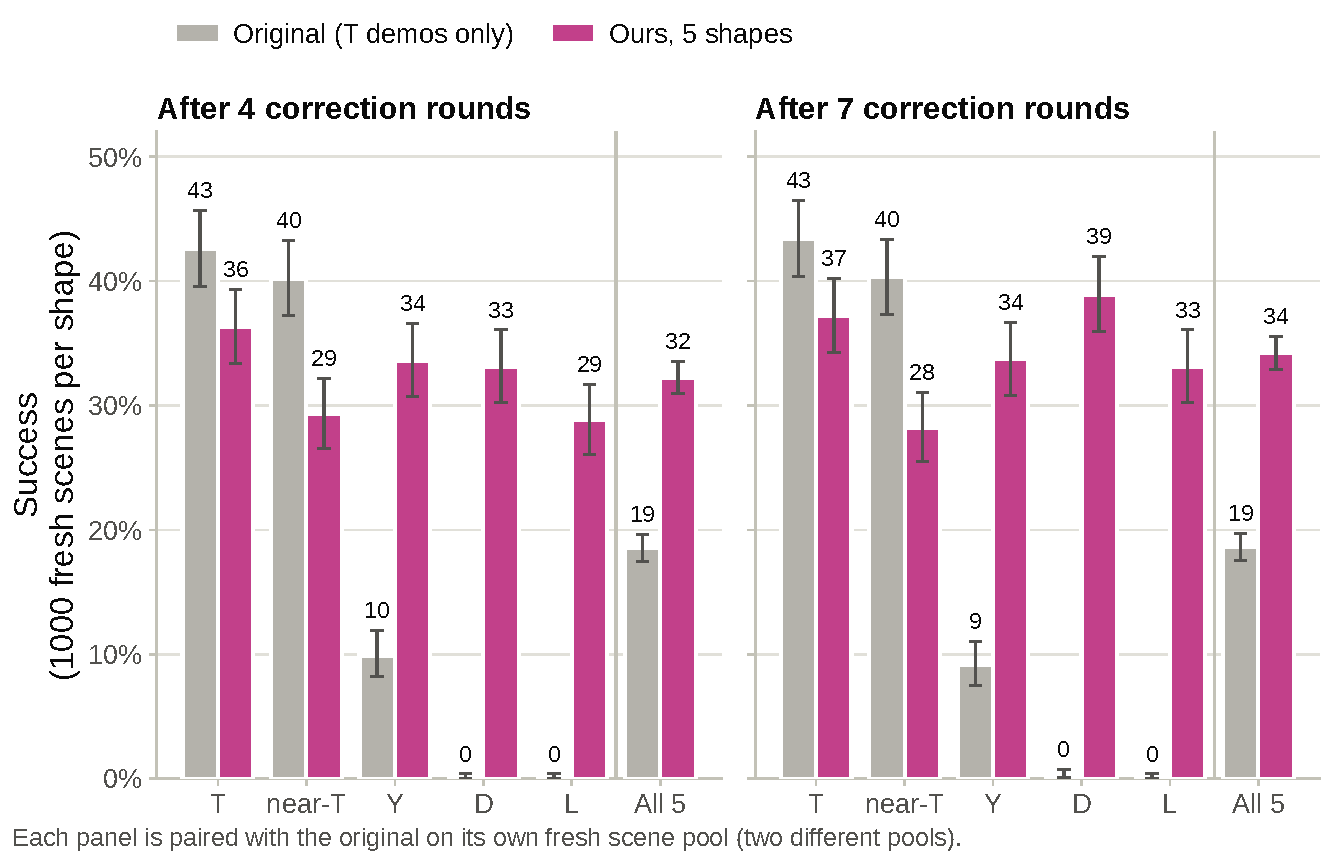
\includegraphics[width=0.48\textwidth]{../figures/final_5shapes_bars.pdf}\hfill
  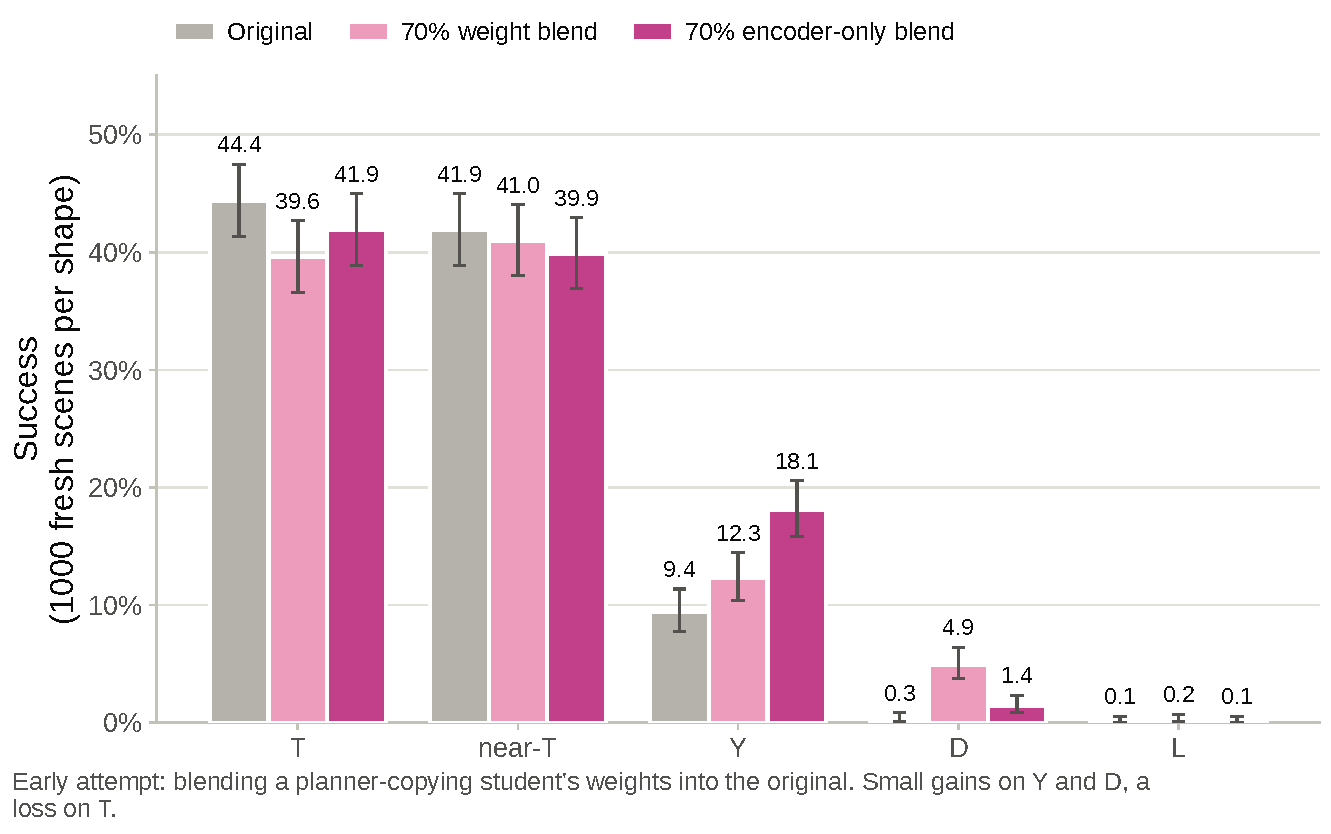
\includegraphics[width=0.48\textwidth]{../figures/final_blends_5shapes.pdf}
  \caption{Left: five-shape students after 4 and 7 correction rounds against the original (two fresh pools). Right:
  the early weight-blend attempt (Section~\ref{sec:negative}).}
  \label{fig:app-blends}
\end{figure}

\begin{figure}[h]
  \centering
  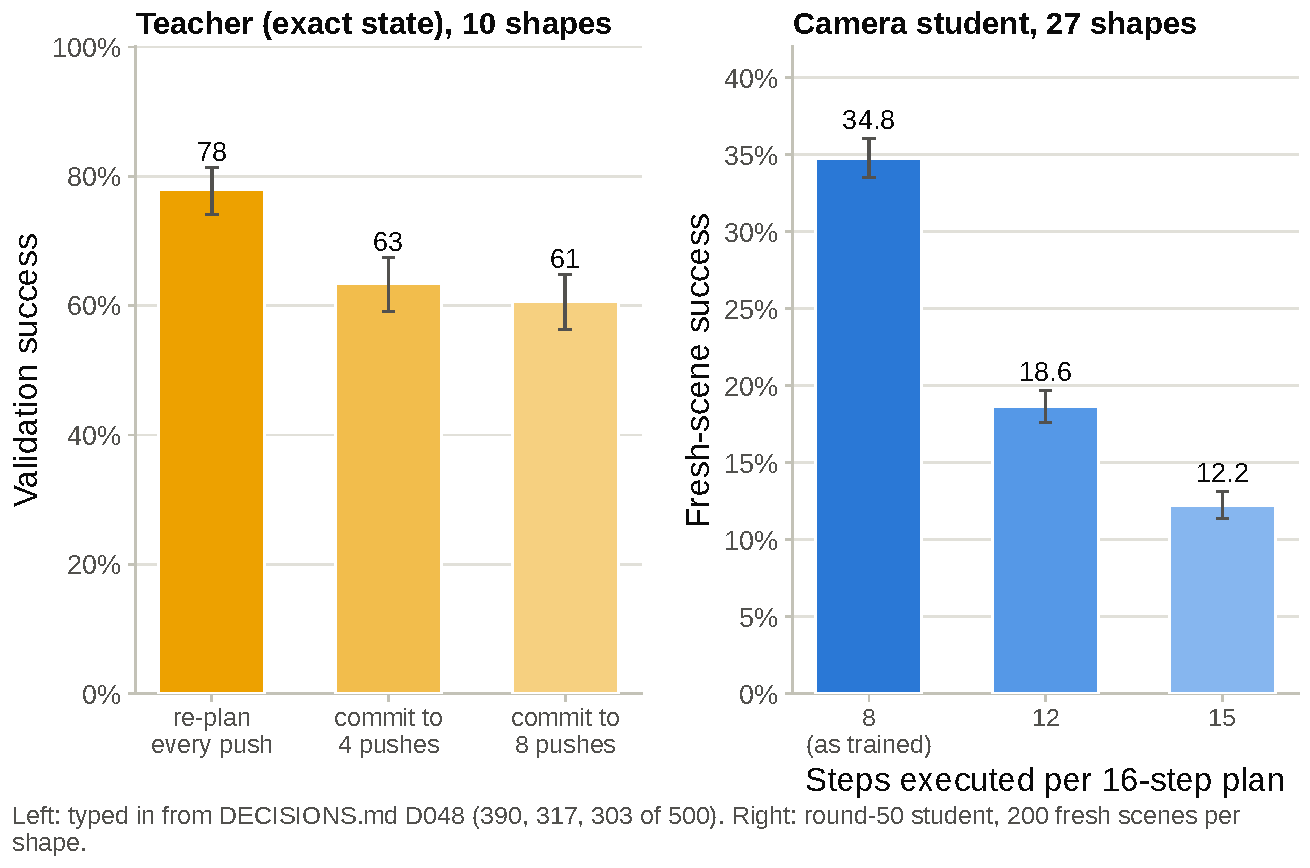
\includegraphics[width=0.48\textwidth]{../figures/analysis_commitment.pdf}\hfill
  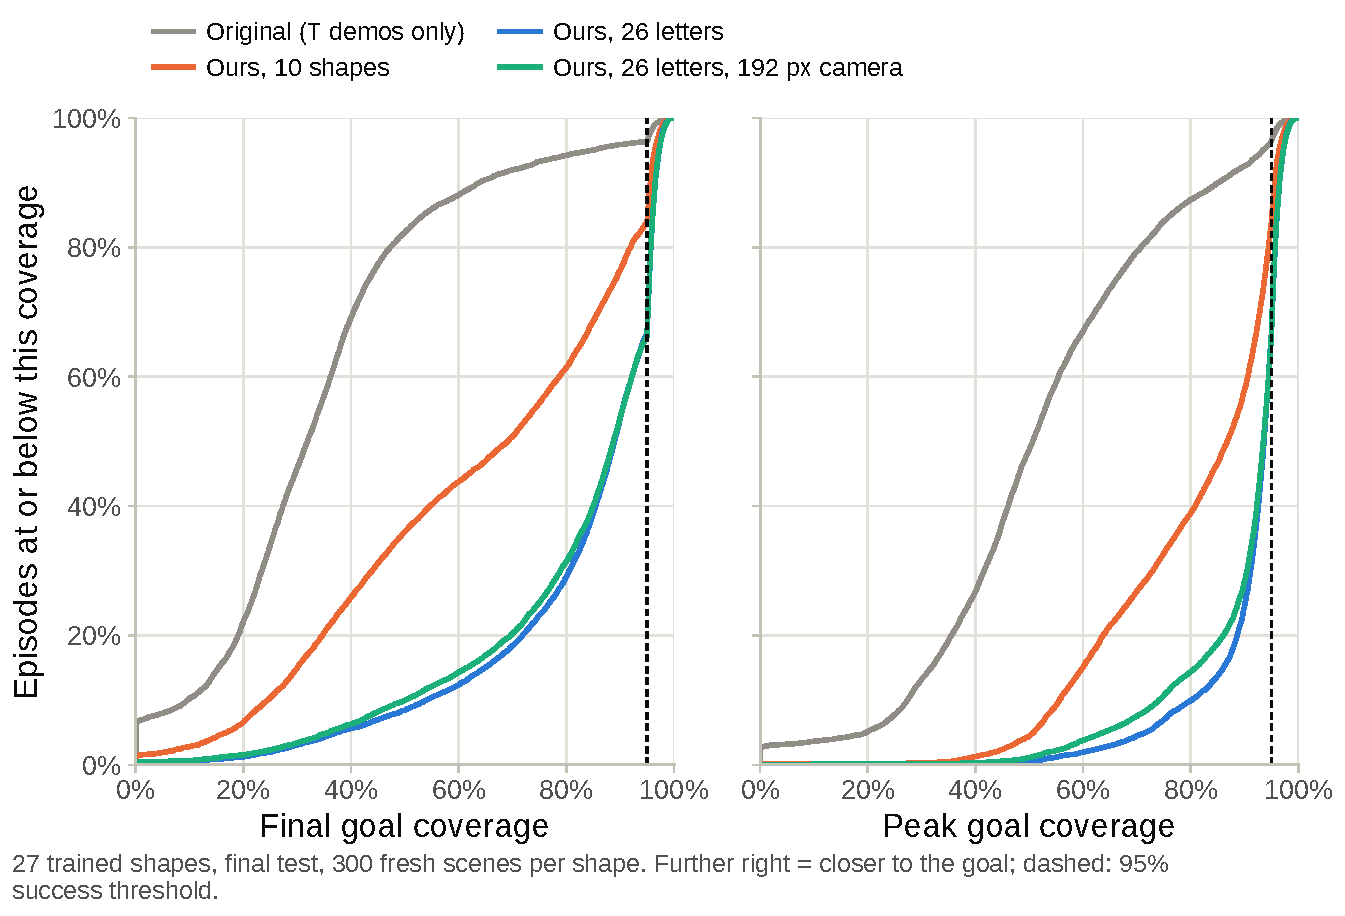
\includegraphics[width=0.48\textwidth]{../figures/coverage_cdf.pdf}
  \caption{Left: committing to more steps per plan hurts both the teacher (reads state) and the camera student. Right:
  cumulative distributions of final and peak coverage for the four policies.}
  \label{fig:app-commit}
\end{figure}

\todo{experiment log summary table (every run, including abandoned ones) and reproduction commands}

\end{document}
